\documentclass[]{aiaa-tc}

\usepackage{authblk}
%\usepackage{subfigmat}
\usepackage{booktabs}
\usepackage{hyperref}
\usepackage{subfig}
\usepackage{amsmath}
\usepackage{amssymb}
\usepackage{pdflscape}
\usepackage{appendix}
\usepackage{pdfpages}
\usepackage{tikz}
\usepackage{geometry}



\newcommand{\bigcell}[2]{\begin{tabular}{@{}#1@{}}#2\end{tabular}}

%\usepackage[margin=3cm]{geometry}

\setlength\extrarowheight{5pt}

\bibliographystyle{aiaa}


\newcommand{\f}{\frac}
\newcommand{\p}{\partial}
\newcommand{\ds}{\displaystyle}
\newcommand{\mb}{\mathbf}
\newcommand{\mbs}{\boldsymbol}


\cfoot{\footnotesize\normalfont
       \thepage\ of \pageref{LastPage}\\
        \ifx\aiaa@papernumber\@empty
          \relax
        \else
          \if@aiaa@handcarry Paper \aiaa@papernumber\fi
        \fi
       }


\begin{document}

  %\maketitle

  \vspace{4em}
  \begin{center}
    A proposal to the NASA ARMD Team Seedling Program: 
    \vspace{2em}

    {\Huge Coupled Aero­-Propulsive-Elastic Design of an Ultra­Light, Highly Flexible, Human Powered Aircraft}

    \vspace{2em}
    submitted to the NASA Aeronautics Research Institute by: 

    \vspace{3em}
    \begin{figure}
        \centering
        
\includegraphics[width=.5\textwidth]{images/seedling_logos}
    \end{figure}
    \vspace{3em}


  \end{center}


  \begin{tabular}{l l}
    Principal Investigator & Justin S. Gray; NASA Glenn Research Center, Propulsion Systems Analysis Branch \\ 
    & \\
    Co-Investigators & Dr. Juan J. Alonso; Stanford University, Department of Aeronautics and Astronautics \\
                     & Dr. Graeme Kennedy; Georgia Institute of Technology, School of Aerospace Engineering \\ 
                     & Dr. Todd Reichert; Vice President of Aerodynamics, AeroVelo Inc. \\
    & \\ 
    Team Members & Cameron Robertson; Vice President of Structures, AeroVelo Inc. \\ 
                 & Jeffrey Chin; NASA Glenn Research Center, Propulsion Systems Analysis Branch \\
                 & Kevin Reynolds; NASA Ames Research Center, Intelligent Systems Branch \\
                 & Anthony Piazza; NASA Armstrong Flight Research Center, Aerostuctures branch \\
  \end{tabular}

  \newpage

  \section{Introduction}

    The Fundamental Aeronautics Program has identified \textbf{Ultra Efficient Commercial Vehicles} as 
    a key research thrust. A number of concepts have been proposed along those lines through the N+2 and N+3 programs, such as 
    the MIT D8 double­-bubble and the Boeing SUGAR­-High truss­-braced wing. These aircraft rely on 
    very high­-aspect ratio, extremely flexible wings to significantly reduce the vehicle's empty weight and help achieve very low energy consumption. 
    Long endurance solar sensorcraft and communication platforms being proposed by companies such as General Atomics,
    Scaled Composites, Google and Facebook, also focus on extreme empty weight reductions to minimize energy consumption, resulting in highly 
    flexible wings. This situation begs the question, \textbf{``How can future aircraft designs be changed to take full 
    advantage of highly flexible structures?''} The Vision 2030 CFD study\cite{vision2030} also highlights the 
    design of highly flexible wings as a modeling grand challenge problem. That study specifically 
    focused on the need for highly multidisciplinary, tightly coupled design processes with high 
    fidelity tools to address this grand challenge.

    Aircraft empty weight reduction is a major driving factor pushing designs toward highly flexible structures. 
    While lower structural weight helps to achieve lower energy consumption it also tends to result in very large 
    deflections, aeroelastic and control issues, and, possibly, highly non-linear structural responses. These characteristics mean that, in addition to the vehicle aerodynamics,
    structural considerations play a major role in the overall approach to aircraft design, and have been shown to be a primary 
    concern for aircraft stability\cite{heliosfailure_2007}. Thus it is interesting to consider the question, 
    \textbf{``Could structural health monitoring technologies be used to enable lighter 
    weight structures?''}, to address the \textbf{Real­-Time System­-Wide Safety Assurance} thrust. 

    One of the major challenges associated with designing highly flexible wings is that the as-flown configuration 
    is dramatically different than the as-built configuration (jig shape). While this difference between the jig shape and the as-flown, 1-g shape is commonly solved in typical commercial aircraft designs by building the jig shape that, under a 1-g load, deforms to the desired cruise shape~\cite{Kennedy:2014:tacs-tripan, Kennedy:2012:CMC, 
      Kennedy:2014:High-aspect-ratio}, new challenges arise when treating highly-flexible
    structures and aircraft that operate at various design conditions (supersonic vehicles, high-endurance high-altitude aircraft, military aircraft, etc.). Besides the non-linear structural 
    response these wings also tend to exhibit different load distributions from conventional wings. Many of the concepts 
    are based on electric propulsion systems with propellers spread across the wing. This can have not only a 
    structural impact, but also an aerodynamic and controllability impact as well. These aspects push the 
    limits of todays most advanced high-fidelity aeroelastic design techniques, which currently rely on linear structural 
    models and don't account for any propulsion interactions, nor do they easily handle constraints on dynamic behavior. 

    Although tools currently exist to address each one of the various modeling challenges, there is not yet a well 
    established method to integrate them all into a cohesive system model and then applying that model to an actual 
    aircraft design process. Moreover, brute-force methods to integrate a number of high-fidelity analysis tools and drive them with an optimizer tend to require such large computational times that they are often useless within typical design processes.  This proposal outlines a unique opportunity for NASA to fill this capability gap
    by developing and integrating the necessary tools and applying them to an aircraft design and flight testing effort performed in close collaboration with AeroVelo Inc., the Georgia 
    Institute of Technology, and Stanford University. In 2013 AeroVelo won the Sikorski Human Powered Helicopter Prize by flying the first human powered helicopter capable of staying aloft for 60 seconds and reaching a minimum altitude of 3 meters, with the center point of the aircraft hovering over a 10-by-10-meter square. 
    Their next human powered aircraft will be built to conquer the Kremer Marathon Challenge; fly a 
    human powered aircraft 26.1 miles in under 1 hour. They have invited a NASA-led team of researchers to 
    participate in this project. 

    A human powered aircraft designed for the Kremer Marathon Challenge makes an excellent test case for the 
    wide range of modeling and design challenges associated with highly flexible wings. 
    The only available power is that of the humans on board, and each one can provide about the 
    same amount of power as a cordless drill. In order to reach the speeds necessary, multiple people will be required. 
    Figure \ref{fig:aerovelo-concept} is the initial AeroVelo concept, which includes three pilots spread across the wing
    span with three propellers. Spreading the pilots out over the wing span yields a distributed load profile (also known as "span loading"), 
    which must be supported by a very light weight and extremely flexible structure. Weight is not the only 
    key design consideration either. To keep aerodynamic drag low, it is critical to maintain laminar flow 
    over as much of the wing as possible and to ensure that the large structural deformations do not cause unnecessary deviations in the aerodynamic performance and the stability of the aircraft. 

    \begin{figure}[!hbt]
        \centering
        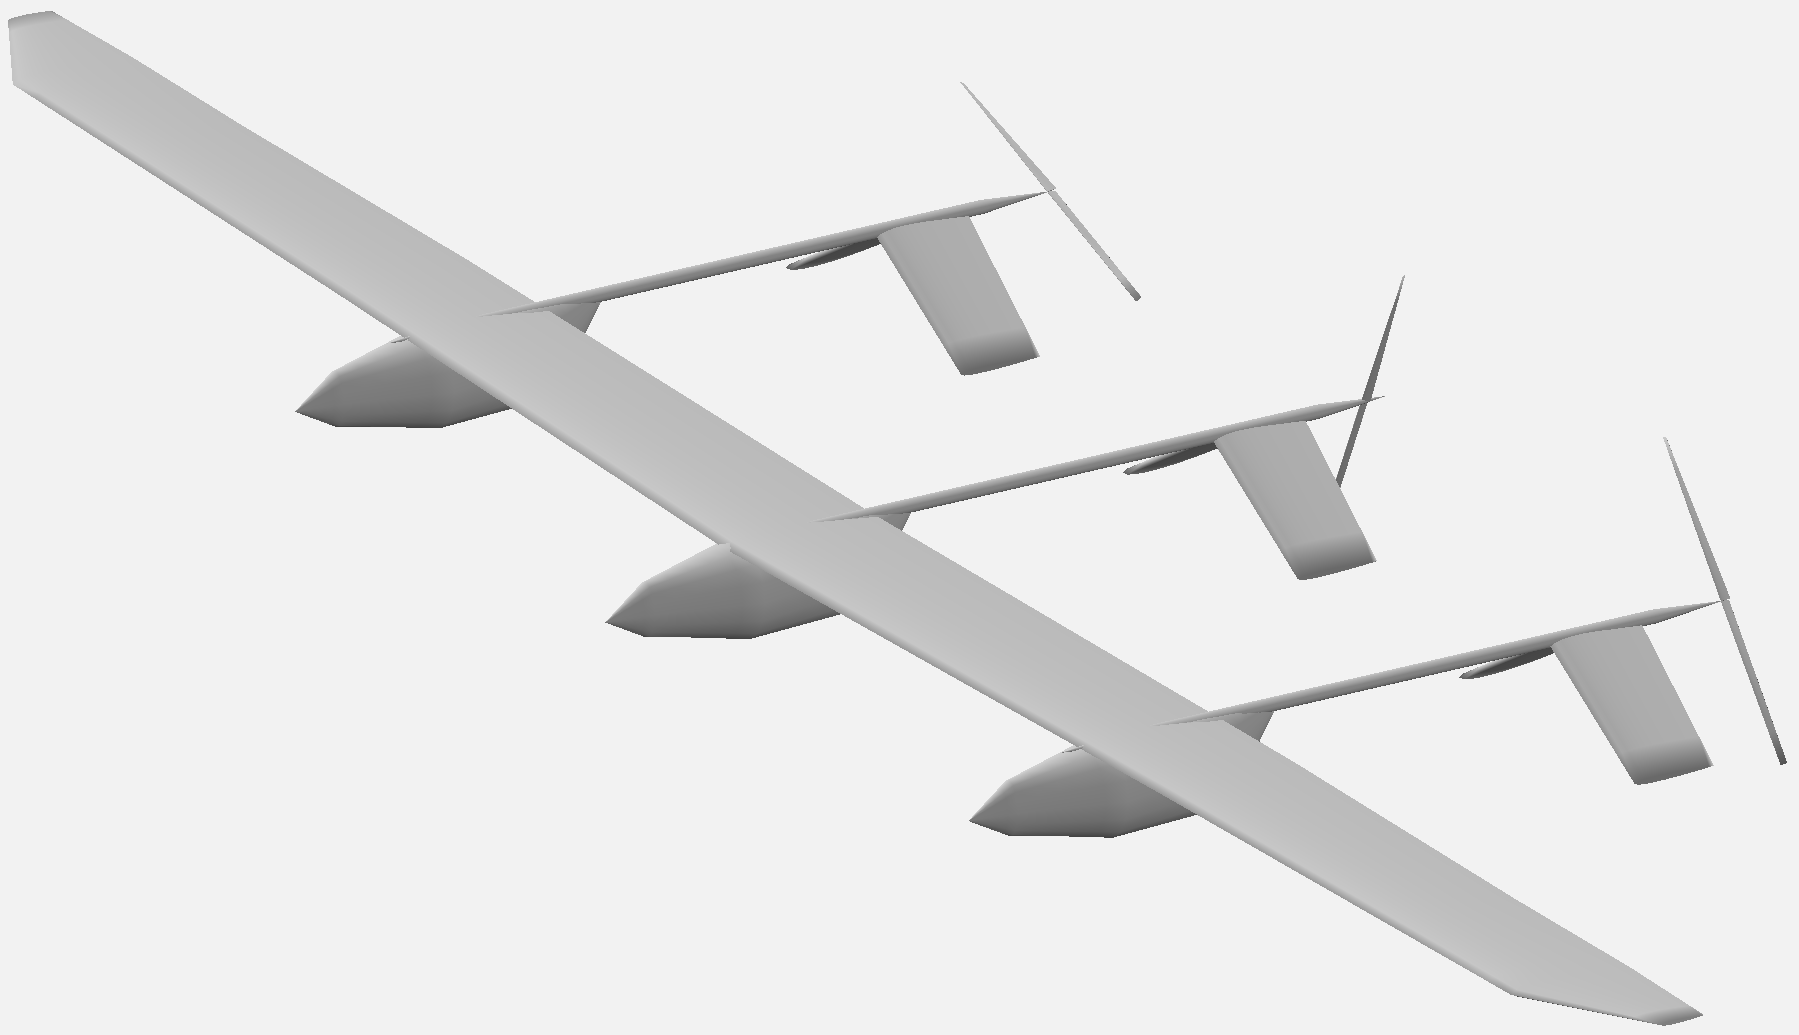
\includegraphics[width=.5\textwidth]{images/vsp_concept_solid}
        \caption{AeroVelo concept of 3-pilot human-powered aircraft for the Kermer Marathon Aircraft}
        \label{fig:aerovelo-concept}
    \end{figure}

    The combination of low speed flight, very low available power, distributed propulsion, and highly 
    flexible span-loaded structures makes this human powered aircraft an excellent analog for 
    high altitude, long endurance aircraft. Hence all of the tools and methods developed under 
    this effort will be directly applicable to that class of aircraft. By working with a human powered 
    aircraft, we are able to achieve a lower cost, rapid feedback environment to develop and validate these 
    new methods. Then later efforts can quickly apply the new methods to design studies of interest to NASA such as the D8, SUGAR,
    or HALE concepts. 

    During Phase I of this effort, the analysis tools and coupled design environment will be built and 
    the detailed design of the Marathon aircraft will be completed. In addition, sub-scale testing will be 
    performed to validate structural models and construction techniques. During the Phase II effort, two 
    parallel efforts will be pursued. First the aircraft will be built, tested, and flown to attempt the Kremer Marathon Challenge. 
    The aircraft will be used as a flying test bed to collect further structural and aerodynamic validation data as well 
    as additional data on flight handling characteristics and overall performance. All the data collected, 
    models generated, and the final detailed design are intended to be released publicly under an open-source license
    upon completion of the challenge. Second, additional research will be conducted to extend the design tools to 
    for the design of a HALE atmospheric satellite aircraft. This additional design effort will leverage all of the experience 
    gained from working on the human powered vehicle and move the work further toward an actual commercial application.   In particular, the ability to utilize the tools and integration methods developed and to include the stability and control requirements for aircraft whose flight altitudes can vary widely (from as low as 10-12 Km to as high as 28 Km in altitude) will be required to tackle such designs.  Moreover, these aircraft are designed, from the ground up, to be highly (if not completely) autonomous.  The proposed Phase II effort will incorporate these concepts of autonomy in our multi-disciplinary design environment, providing a valuable test case and database for future efforts in autonomous aircraft design within NASA.

  \section{Objectives and Technical Approach}

    The overall objective of this work is to design, test, and fly a human powered aircraft, 
    capable of flying 26.1 miles in under 1 hour using state-of-the-art multidisciplinary 
    design optimization techniques. In order to make this happen, we will also develop a novel integrated 
    design environment, based on a collection tools with analytic gradients (OpenMDAO, SU2, SUave 
    modules, TACS, etc.) that can result in optimal aircraft designs with a degree of confidence far beyond 
    what is typical of conceptual tools.   While during this work the design environment will be used in the 
    context of a human-powered aircraft,  the intent is to ensure that the methods will continue to be used 
    for advanced, low-fuel consumption aircraft concepts of interest to NASA.  The specific design that we will 
    pursue will be performed with fully-coupled aerodynamic, non-linear structural, and propeller models. Working 
    in the context of a full aircraft design process, from conceptual all the way to detailed design, 
    provides a unique opportunity to apply multidisciplinary optimization methods and validate
    the results within a vary small time frame. 

    Phase I of the work will focus on the design of the aircraft and the design environment used 
    to accomplish this goal. NASA Glenn Research Center, 
    NASA Ames Research Center, Stanford, and the Georgia Institute of Technology will be responsible 
    for collaboratively developing the propulsion, aerodynamic, and structural analysis 
    models needed as well as integrating them together to perform the coupled analysis. AeroVelo will
    use the models to perform the conceptual, preliminary, and detailed design of the actual marathon 
    aircraft in very close collaboration with the other partners. NASA Glenn Research Center, 
    The Georgia Institute of Technology, and AeroVelo will all collaborate on a set of structural validation 
    tests designed to validate the tool sets and construction methods needed for the aircraft.  Stanford 
    University will be responsible for the aerodynamic modeling portions of the work, as well as 
    help with the integration of tools and the overall organization of the multidisciplinary design 
    procedure that will be used for this work.

    \subsection{Model Integration}

    NASA Glenn will be responsible for managing the integration of the various analyses into 
    a single system model via the OpenMDAO framework. OpenMDAO provides advanced 
    capabilities for high-fidelity code coupling. These capabilities will be leveraged to combine the geometry,
    propeller, wing aerodynamics, and structural models into a single coupled aircraft model. The aircraft 
    model will the be used as a design tool by AeroVelo to facilitate the actual design process. 
    Figure ~\ref{fig:n2} shows details of how the multidisciplinary coupling will be set up. The aerodynamics 
    and structures disciplines will both be implemented using high fidelity models. The propeller modeling 
    will be accomplished with a combination of low and high fidelity models. The use of high fidelity models 
    will pose a significant challenge to the design process. Airfoils must be designed independently along the propeller and
    across the entire wing. The wing planform and the propeller chord and twist distributions must also be selected.  In addition, material thicknesses throughout the structure
    will be sized independently. The combination of aerodynamic and structural design variables 
    can easily number in the 100's to 1000's. With such a large design space, gradient-based optimization 
    combined with adjoint analytic derivatives are the most effective tool for navigating the design space. 

    \begin{figure} \centering
        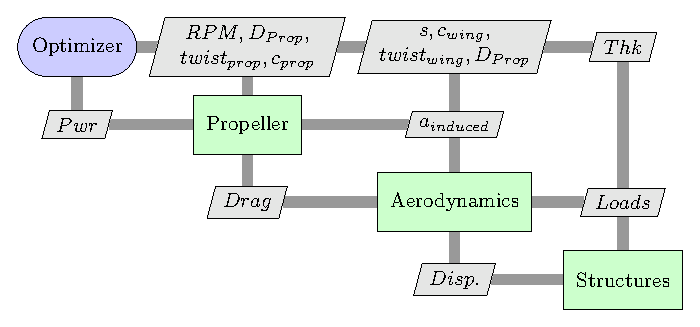
\includegraphics[width=.75\textwidth]{xdsm/overall}
        \caption{Data flow for the aircraft design process, with coupling between the propeller and aerodynamics models 
        and between the aerodynamics and structural models. }
        \label{fig:n2}
    \end{figure}

    Because of the size of the design space, and larger number of coupled disciplines, OpenMDAO's built in support for 
    automatic system-level coupled derivatives will be key to building the aircraft-level model. OpenMDAO allows for 
    pure analytic or semi-analytic derivatives, using both forward and adjoint formulation. The effectiveness of OpenMDAO's 
    derivative capability has been successfully demonstrated on two different design problems that are similar in complexity 
    and scale to the proposed human powered aircraft design: A small satellite design and an aero-structural 
    wind turbine design\cite{gray2014derivatives}. The small satellite design problem had over 25,000 design variables 
    and over 30 disciplines. This problem demonstrated OpenMDAO's capabilities to solve problems of very large scale with adjoint 
    derivatives. The aero-structural design of a wind turbine was a very different problem. It used a mixture of analytic and 
    finite difference gradients with a complex system level model considering aerodynamics, structures, and economics. 
    This problem showed that even when applying finite difference to some of the disciplines for gradients, the analytic 
    derivative approach yielded a factor of 5 reduction in compute costs. This previous work demonstrates the 
    value of OpenMDAO's analytic derivatives capability and highlights why it will be a central feature in the design 
    optimization for a human powered aircraft. 

    By using the OpenMDAO framework, the modeling methods will be built in a modular fashion that will allow a wide range of
    different analysis tools to be used. This will help extend the applications of the work to other types of aircraft beyond the 
    initial human powered aircraft and will make extension to HALE applications in year 2 strait forward. 

    % During the process of setting up the entire framework for the high-fidelity design of the human-powered vehicle, it might become necessary to resort to hierarchical decomposition schemes, such as Collaborative Optimization (CO), where the overall design problem is decomposed into a number of optimization subproblems coordinated by system-level optimizer.  Such hierarchical optimization architectures can greatly decrease the cost of the overall optimization problem and, furthermore, can enable the computation of performance measures and their sensitivities, in each participating discipline, to proceed along in parallel, thus decreasing the overall clock time required to carry out a design.  Given that all the high-fidelity modules will become part of the OpenMDAO environment, it becomes straightforward to re-organize the design problem in a manner that renders it tractable.  Such system-level optimization approaches will be tried under the leadership of NASA Glenn Research Center and with participation from Stanford University. (**** Add a task for this?  Something like: "Hierarchical Decomposition Schemes for High-Fidelity Optimization"? ****)


    \subsection{Aerodynamic Modeling}

\noindent Over the course of the past 8 years~\cite{Palacios:Adjoint-Based,Choi:2008qf}, our team has developed a comprehensive framework for the aerodynamic shape optimization of arbitrary aircraft configurations that can effectively deal with both aerodynamic performance and stability \& control considerations.  This framework is embodied in the Stanford University Unstructured (SU2) software suite~\cite{palacios2013}, which was developed for the specific task of solving PDE analyses and PDE-constrained optimization problems on arbitrary unstructured meshes. While the framework is general and is meant to be extensible to arbitrary multi-physics problems, the core of the suite is a Reynolds-averaged Navier--Stokes (RANS) solver capable of simulating compressible, turbulent flows (using both the Spalart--Allmaras and SST turbulence models) that are characteristic of typical problems in aerospace engineering. SU$^2$ was constructed with aerodynamic shape optimization problems in mind, and therefore, adjoint-based sensitivity analysis is a key feature that is built directly into the RANS solver.

In particular, the adjoint methodologies that we have included in the SU2 suite enable us to, very rapidly, obtain surface sensitivities of cost / constraint functions related to the solution of the CFD problem with respect to an arbitrary number of parameters.  In fact, the sensitivity formulation in SU2, which will be leveraged by the OpenMDAO framework, is based on a surface formulation that bypasses the need to perturb the volume mesh during the process of computing the individual adjoint-based gradients, resulting in a great reduction in the overall cost of the sensitivity procedure, and imposing no limitations on the number of design parameters that an optimization problem might include.

%
As can be seen in Fig.~\ref{fig:sketch}, the fluid domain $\Omega$ is bounded by a disconnected boundary $\delta \Omega$ that is divided into a ``far-field'' component, $\Gamma_\infty$, and a solid wall boundary, $S$. $\Omega$ has been further divided into two subdomains $\Omega_i$ and $\Omega_o$ separated by the ``near-field'' boundary $\Gamma_{nf}$. Note that $\Gamma_{nf}$ remains fixed throughout the optimization process, but the solid surface $S$ changes as needed to meet the optimization criteria.  The fact that we highlight the near-field boundary in the formulation is simply so that it is clear that the formulation can be extended to include surface integrals over arbitrary surfaces contained in the domain, which do not necessarily coincide with the surface of the aircraft.  This is the case, for example, when supersonic boom functions are differentiated, as is the case in supersonic aircraft design, the problem we use to illustrate the features of SU2.
%
\begin{figure}
  \begin{center}
	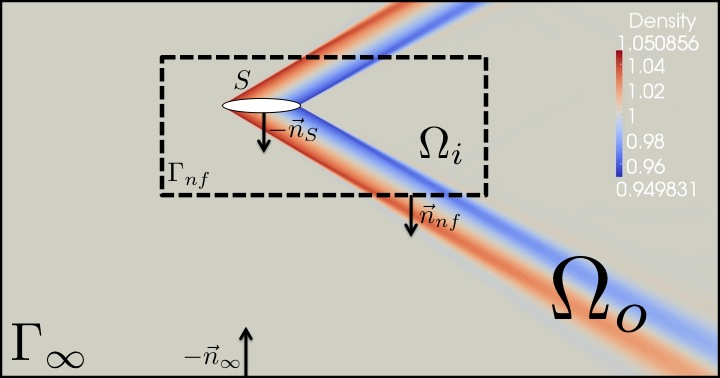
\includegraphics[bb = 0 0 720 378,width=0.56\textwidth]{images/sketch.jpg}
	\caption{Schematic view of the configuration with near-field and far-field boundaries.}\label{fig:sketch}
  \end{center}
\end{figure}
%
%
A typical optimization problem seeks the minimization of a certain cost function $J$ with respect to changes in the shape of the boundary $S$. We focus on functionals defined as integrals over the solid surface $S$, and integrals over the near-field boundary $\Gamma_{nf}$,
\begin{equation}
J =\int_S{\vec d \cdot (P \vec n_S)\,ds}+\int_{\Gamma_{nf}}{g(x,P)\,ds} = \int_S{j_S\,ds}+\int_{\Gamma_{nf}}{j_{nf}\,ds},
\end{equation}
where $P$ is the value of the pressure, $\vec n_S$ is a normal vector to the solid surface $S$ pointing outside the domain, $g(x, P)$ is a function that depends on the spatial coordinates and the pressure at the near-field, and $\vec d$ is an arbitrary constant vector. We stress that this formulation has been shown to enable all of the tasks that we have encountered in aircraft design, including, for example, supersonic aerodynamic and low-boom design, using equivalent area distributions. The goal is to efficiently compute the variation of the above functional caused by arbitrary (and multiple) deformations of $S$.
%
Upon an infinitesimal deformation $\delta S$ of the control surface $S$ along the normal direction $\vec n_S$, the cost function varies due to the changes in the solution induced by the deformation:
\begin{eqnarray} \label{objvar}
\delta J &=&  \int_S{\vec d \cdot \delta P \vec n_S \,ds} + \int_{\Gamma_{nf}}{\frac{\partial g(x,P)}{\partial P}\delta P\,ds}  + \int_{S}{(\vec d\cdot\vec\nabla P )\delta S \,ds}.
\end{eqnarray}
%
In the last expression we note that the objective function variation depends on the linearized steady RANS flow equations, $\vec\nabla \cdot (\vec \delta F) = 0$, where $\vec F$ are the convective and viscous fluxes. We resort to the adjoint state $\Psi =(\psi_1, \vec \varphi, \psi_5 )$ to tackle the variation of the flow variables $\delta P$ in the objective function:
\begin{eqnarray}
\delta J &=&\int_S{(\vec d \cdot \vec n_S)\delta P  \,ds} - \int_{S}{(\vec n_S\cdot\vec \varphi) \delta P\,ds} + \int_{\Gamma_{nf}}{\frac{\partial g(x,P)}{\partial P}\delta P\,ds}  -  \int_{\Gamma_{nf}}{\Delta \Psi \left(\vec n_{nf} \vec A\right)\delta U\,ds} \nonumber \\
&+& \int_{S}{\left(\vec d\cdot\vec\nabla P + (\partial_n \vec v\cdot \vec n_S)\,\vartheta+\nabla_S(\vec v \,\vartheta )\right)\delta S\,ds},
\end{eqnarray}
where $\Delta \Psi = \Psi_i-\Psi_o$ is the difference between the values of $\Psi$ above and below the near-field boundary, $\vec A$ is the Jacobian matrix of the fluxes, and $\vartheta = (\rho \psi_1+\rho\vec v\cdot \vec\varphi+\rho H\psi_5)$. Finally, the following adjoint system should be solved
\begin{equation}
\vec A^T  \cdot \vec \nabla \Psi= 0.
\end{equation}
where the appropriate boundary equations are included for all boundaries, including those that are used to represent the propulsion system effects.  In previous work~\cite{Palacios:Adjoint-Based} we have also shown how this methodology can be extended to treat functionals of the equivalent area distribution of a full aircraft computed with detailed CFD.

Our work in SU$^2$ has been released under an open-source license, and it is freely available to the community, so that developers around the world can continue to verify, validate, contribute to the source code, and further improve the accuracy and capabilities of the suite. This open-release policy make SU2 ideally suited to interface with other open-source tools in the work propose here.  The RANS capabilities in SU$^2$ have been carefully validated with a number of different test cases~\cite{SU2:Scitech2014}, and have been used extensively for the calculation of flows over supersonic aircraft configurations during the NASA N+2 and Low-Boom Flight Demonstrator programs.  Fig.~\ref{fig:lbfd} below shows some recent analyses and optimizations completed with SU$^2$ that are representative of the configurations that will be analyzed in the proposed work.
%
\begin{figure}[h]
\parbox{\textwidth}{
\parbox{8.0cm}{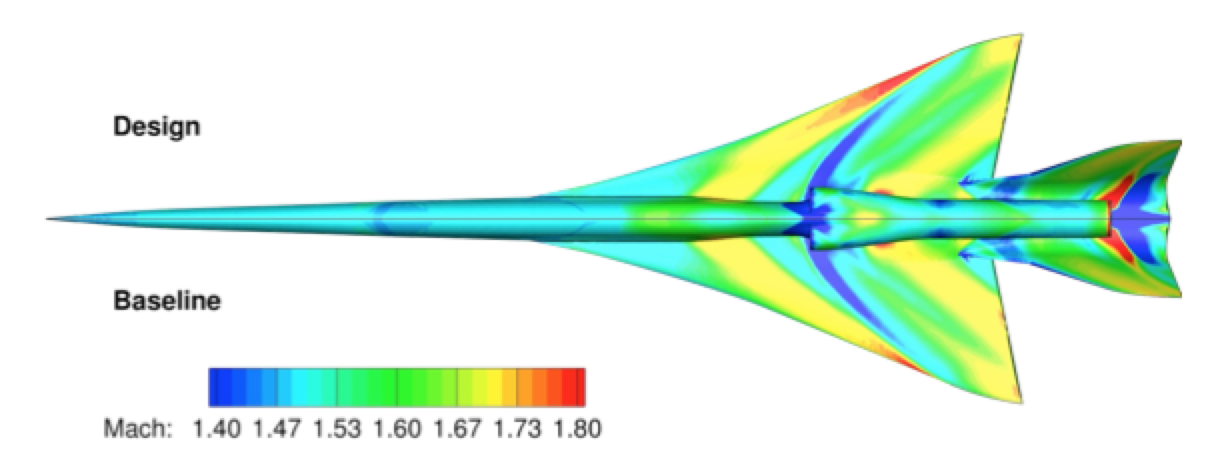
\includegraphics[width=8.0cm]{images/lbfd1} \\ Result of baseline analysis and optimization for low-boom flight demonstrator concept.}\hfill\parbox{8.0cm}{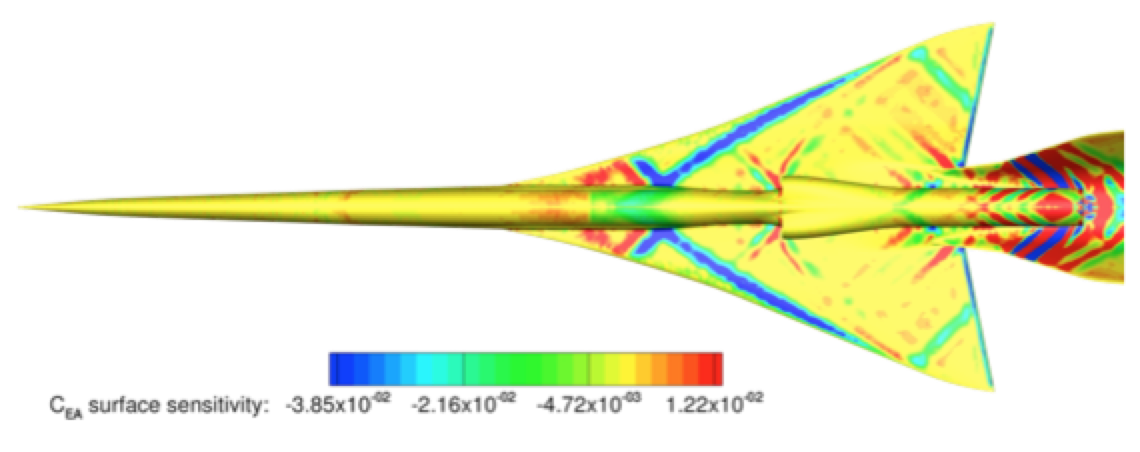
\includegraphics[width=8.0cm]{images/lbfd2} \\ Surface sensitivity map for equivalent area distribution.}}
\caption{Sample SU$^2$ RANS calculations and design optimizations for a low-boom flight demonstrator concept, as well as surface sensitivity maps for a function of the aircraft equivalent area distribution.}
\label{fig:lbfd}
\end{figure}

Given the success of our existing methods, and for purposes of this Seedling effort, we consider the capabilities of the SU$^2$ framework to be sufficient as they currently exist, and no further improvements are necessary to be able to deal with aerodynamic performance and stability \& control predictions.  This shape optimization capability, however, must now work in concert with the aero-structural analysis of our advanced concepts.  These additional interactions must be accounted for in the development of system-level sensitivities and a majority of the effort in this section will be directed towards the enabling of multidisciplinary capabilities in the SU$^2$ framework.  As discussed later in this proposal using the example of an aerostructural optimization, the majority of the SU2 effort envisioned during Phase I will include the development of all necessary sensitivities and partial derivatives that are required to couple SU2 with the TACS solver and its adjoint, should that task become necessary.

    \subsubsection{Propeller Analysis}
    
    For the analysis and design of the propellers in our vehicle, we intend to use a multi-fidelity approach that relies on a hierarchy of two separate solution (analysis and optimization) procedures: a low-fidelity and a high-fidelity approaches.
    
    Two options are being considered for the lower fidelity propeller analytsis. One option is the low-fidelity propeller analysis and design module in the SUave (Stanford University aerospace vehicle environment) environment, which is based on the work of Adkins \& Liebeck~\cite{Adkins:Design}.  A second option is Ning's blade element momentum based method designed specifically for use with optimization, 
    CCBlade\cite{NING:BEM}. 

    These methods use airfoil drag polar data at various Reynolds and Mach numbers and construct the optimal propeller shape (chord and twist distribution) that result in a minimum induced loss design. Airfoil drag polar data will be generated using XFOIL, which provides rapid and accurate models for 2D airfoil performance. 
    Using these procedures, propellers can be sized and optimized very rapidly and sensitivities of the optimum performance can be obtained and interfaced with OpenMDAO for further analysis.
    
    In addition, and while the low-fidelity model is expected to be relatively accurate if sufficient drag polar data is provided, to resolve higher-fidelity effects we will also leverage SU2.  SU2 is able to solve (and provide sensitivities) for computations performed in a rotating coordinate frame, as would be the case for an isolated propeller.  In such a frame of reference, the problem is rendered steady, and the same methodologies described earlier and contained within SU2 can be used to analyze and optimize a design.

    The combination of these two models of different fidelities will be accomplished using an additive correction anchored on the results of the low-fidelity model.  The additive correction can be computed across the entire design space using the smallest possible number of evaluations of the high-fidelity model (and possibly gradients) and fitted using Gaussian Process Regression.  The part of our team at Stanford University already has significant experience with this methodology and will leverage existing libraries to carry out this work.

    The propeller design will be performed as part of the overall aircraft design optimization. RPM, radius, twist and chord distribution, and 
    physical location will all be considered as design variables. Using the combination of low and high fidelity analyses, the propeller 
    effects on the airframe and vice versa will be considered. Propulsive loads on the airframe will be modeled, and aerodynamic affects of the
    airframe on the propeller will also be accounted for. As mentioned earlier, SU2 has has preliminary support for actuator 
    disk boundary conditions that will be needed to implement the coupled wing­-propeller design process. The actuator disk model is based on a radially-varying prediction using a blade-element-momentum theory approach. The methodology has been demonstrated to work in the low 
    Mach conditions that will be seen by this aircraft. Because it is part of SU2, the actuator disk methodology also provides adjoint derivatives 
    which are fundamental to the application of state-of-the-art gradient based design optimization methods. Researchers at Stanford will be responsible for building for developing the aerodynamic models of the wing and will collaborate with NASA Ames on developing the 
    propeller models. 

    \subsubsection{Wing, Fuselage \& Empennage Analysis}
    
    Similarly to the analysis and design of the propellers, a multi-fidelity approach will be used for the analysis and design of the main elements of the configuration: the wing, fuselage and empennage.  A combination of low-and high-fidelity approaches will be investigated to provide results of high fidelity at the minimum possible computational cost.  In particular, the tools we will use are:
%
    \begin{itemize}
    \item Low-fidelity method: for rapid turnaround of aerodynamic calculations we will use a panel code, TriPan, which, together with reasonably accurate airfoil drag polar information can lead to reasonably-accurate estimates of the performance of the vehicle.  Component interactions, particularly when viscosity is concerned, are not captured very accurately, but such issues can be dealt with in a  multi-fidelity approach.
    \item High-fidelity method: a full RANS low solver will be utilized for the high-fidelity simulations of the entire vehicle.  Details of SU2 have been provided before.
    \end{itemize}
    %
    Given that both SU2 and TriPan are able to provide sensitivity information at relatively low cost, we intend to leverage the availability (and abundance) of gradients to further reduce the cost of creating the Gaussian Process Regression multi-fidelity surrogate models.

    Note that the extent of laminar flow is a fundamental design requirement to attain the required level of performance.  For this purpose, and so that transition can be captured accurately for these configurations, we will use the model of Langtry and Menter~\cite{Langtry:Correlation} that has already been implemented in SU2.  Using such models we can have a reasonable expectation of capturing the effects of transition and laminar flow across the entire configuration.          

 
    
        \subsection{Structural Modeling}

The modeling and design of slender lightweight flexible structures for
human and electric-powered aircraft requires specialized tools due to
the strongly-coupled multidisciplinary physics that govern these
vehicles. These requirements will be met, in part, by performing the
structural modeling with the Toolkit for Analysis and of Composite
Structures (TACS)~\cite{Kennedy:2014:TACS,
  Kennedy:2014:tacs-tripan}. TACS has the necessary capabilities to
develop a tightly integrated multidisciplinary framework for dynamic
and static aeroelastic design optimization. These advanced
capabilities include adjoint derivative evaluation and efficient
parallel load and displacement transfer required for coupled
aeroelastic analysis and design.  In addition, TACS also has support
for isogeometric elements which will reduce the overall computational
cost of the structural analysis. Researchers at the Georgia Institute
of Technology will be responsible for building the structural models
and providing support for integrating them into the OpenMDAO
framework.

One of the key difficulties with incorporating conventional
high-fidelity nonlinear finite-element structural analysis early in
the design process is the high computational cost of
analysis. Isogeometric analysis (IGA) techniques offer a potential
solution to this difficulty by greatly reducing the number of
structural degrees of freedom required to achieve the necessary level
of accuracy. This reduction is especially beneficial in the context of
nonlinear analysis where multiple residual evaluations and linear
system solutions are required for a single analysis.
 
IGA methods utilize the underlying b-spline and NURBS basis functions
from the geometry model for displacement interpolation, producing
smooth and accurate displacement and stress solutions.  This
construction offers two benefits within the context of structural
design optimization. First, IGA methods enable CAD-compatible geometry
modification, ensuring that the final design can be used within
CAD. This is not always possible with general finite-element shape
optimization methods such as free-form-deformation
(FFD)~\cite{Sederberg:1986:FFD, Kenway:2010:CAD}.  Second, IGA
techniques are high-order with superior smoothness properties compared
to traditional finite-element techniques. The resulting smooth
displacement and stress distributions produces a more-favorable design
space for stress-constrained design using gradient-based optimization
methods.

\subsubsection{Nonlinear structural modeling}

In this work, we will utilize a third-order isogeometric shell
elements for nonlinear structural analysis and design.  This IGA-based
element balances the computational costs of analysis and gradient
evaluation, with the superior accuracy of higher-order
elements. However, quadratic b-spline elements are susceptible to both
shear and membrane locking~\cite{Babuska:1992:OLR,
  Chapelle.Bathe}. Therefore, to alleviate this locking issue, we will
utilize a mixed-interpolation of tensorial (MITC)
approach~\cite{Dvorkin:1984:CMB, Bucalem:1993:HOM}.

\begin{figure}[h]
  \centering
  \subfloat[Shell formulation]{
    \label{fig:shell-geometry}
    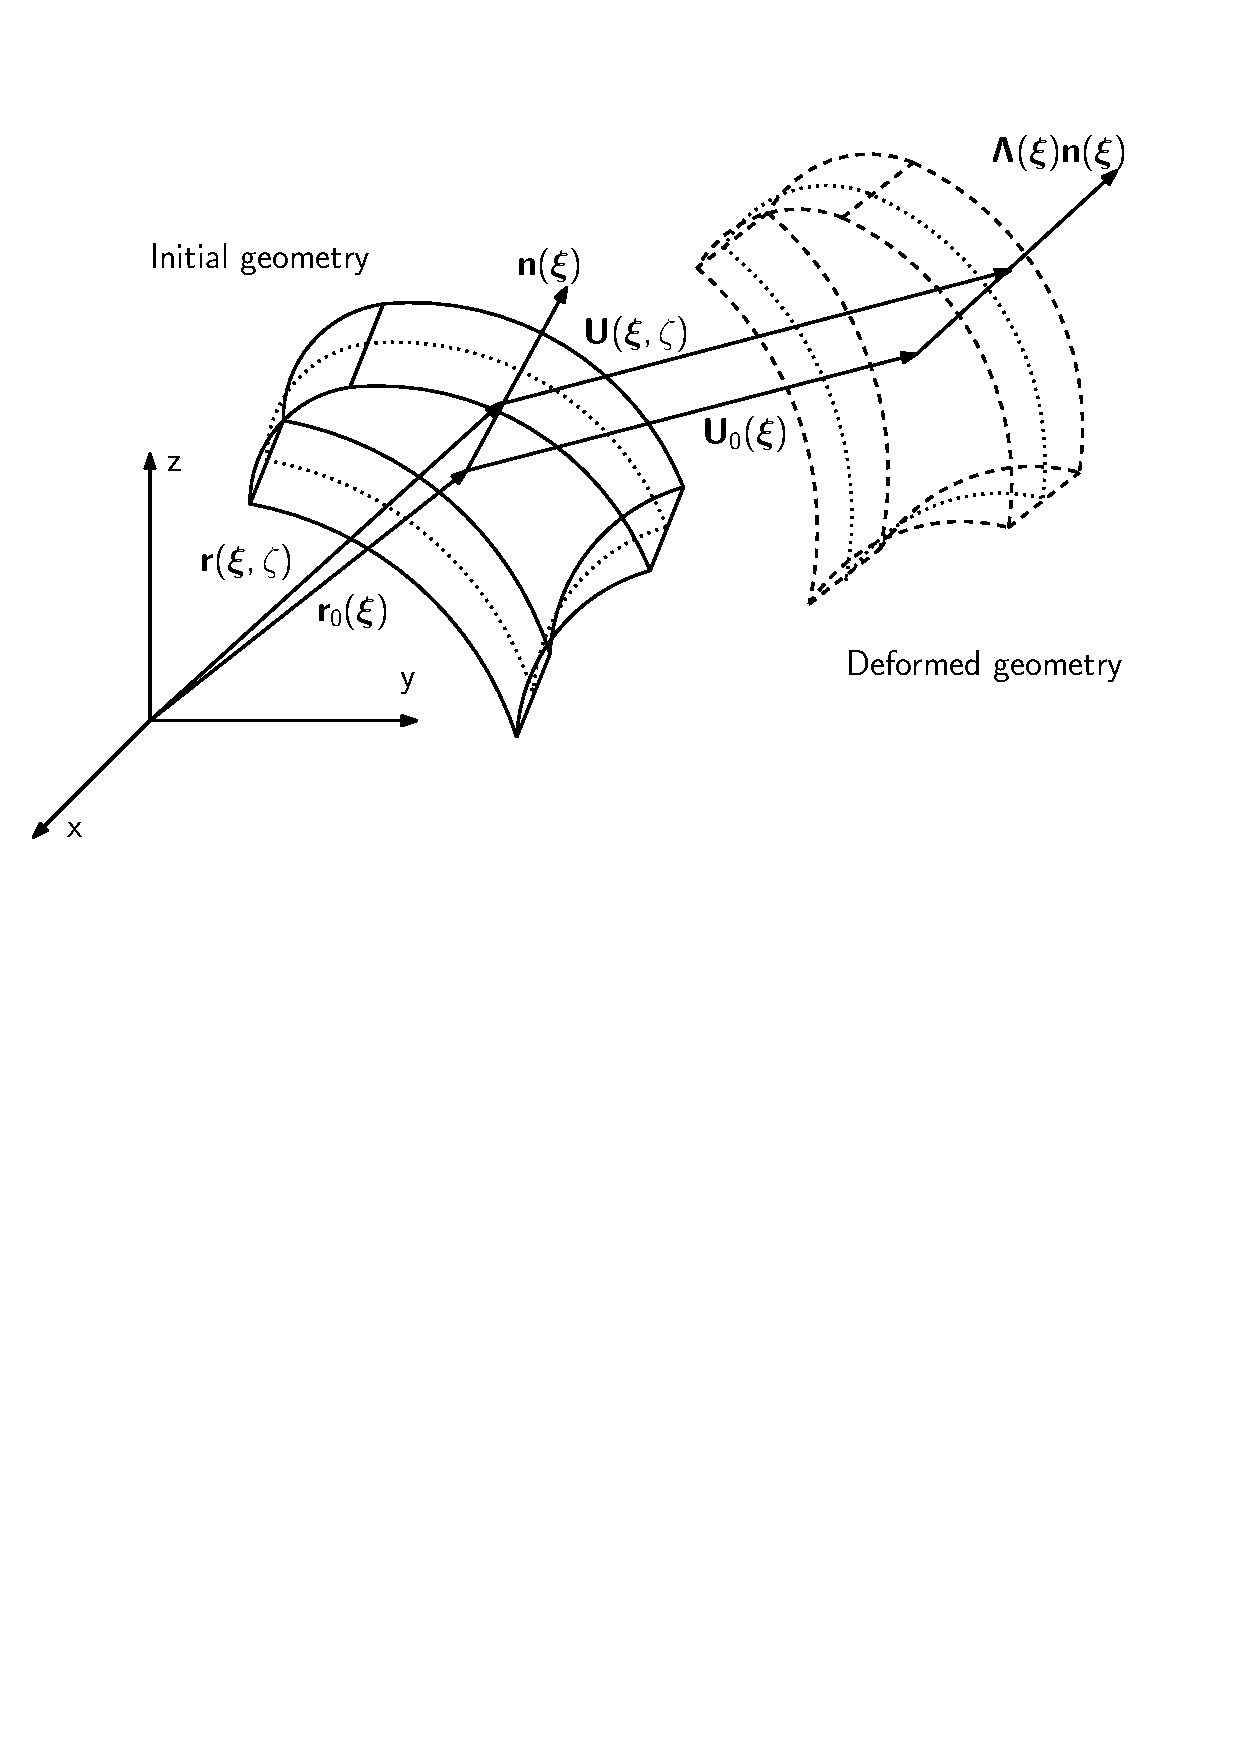
\includegraphics[width=0.4\textwidth]{images/shell_formulation}}
  \subfloat[MITC scheme]{
    \label{fig:mitc-formulation}
    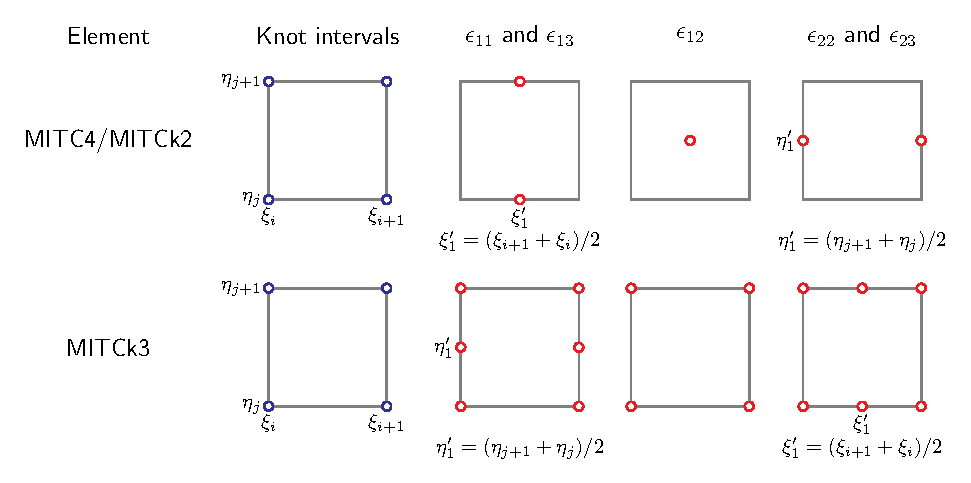
\includegraphics[width=0.6\textwidth]{images/mitc_iga}}
  \caption{The large rotation shell formulation and the b-spline
    compatible MITC scheme.}
  \label{fig:shell-figs}
\end{figure}

The formulation of a general shell element for geometrically nonlinear
analysis to meet accuracy, locking and rigid-body translation
requirements is challenging. To address these issues, we will use a
degenerated solid shell element formulation in which the element is
formulated by reducing the full three-dimensional equations of
elasticity to the mid-surface using shell-theory-like assumptions
about the through-thickness displacement
distribution~\cite{Ahmad:1970:ATS, Bathe:1980:GMN, Parisch:1978:GNA,
  Hughes:1981:NFE}.  The degenerated solid technique is mathematically
equivalent to a shell theory formulation under similar modeling
assumptions~\cite{Buechter:1992:STD}. In addition, we will use an
explicit integration of the strain energy through the thickness,
enabling the direct use of the classical first-order deformation
theory (FSDT) constitutive relationships~\cite{Milford:1986:DIF,
  Buechter:1992:STD}. The in-plane drilling degree of freedom will be
included with a penalization technique to ensure compatibility with
the in-plane displacements~\cite{Hughes:1989:DDF, Simo:1992:FFE,
  Fox:1992:DRF}. This formulation facilitates shell-shell
intersections.

The initial, undeformed shell geometry is represented in terms of the
mid-surface vector, $\mb{r}_{0}(\mbs{\xi}) \in \mathbb{R}^{3}$, and
the unit normal, $\mb{n}(\mbs{\xi})$, that are written in terms of the
local shell coordinates $\mbs{\xi}$. The through-thickness coordinate
is given by $\zeta$. The entire shell volume can be expressed as
follows:
%
\begin{equation} 
  \mb{r}(\mbs{\xi}, \zeta) = 
  \mb{r}_{0} + \zeta \mb{n}, 
  \qquad \mbs{\xi} \in \Omega \subset \mathbb{R}^{2}, \qquad.
  \label{eqn:mid-surface}
\end{equation}
Figure~\ref{fig:shell-geometry} illustrates the initial and the deformed
configurations of a shell segment. 

For the shell model, we use kinematic assumptions that are consistent
with a large-displacement, finite-rotation shell. In particular, we
use a director-field representation~\cite{Simo:1989:SRG1}, such that
the normal deforms as, $\mb{d} = \mbs{\Lambda} \mb{n}$, where
$\mbs{\Lambda} \in SO(3)$ is a rotation matrix. The through-thickness
displacement is written in terms follows:
%
\begin{equation*}
  \label{eqn:displacement-field}
  \mb{U}(\mbs{\xi}, \zeta) = \mb{U}_{0} + \zeta (\mbs{\Lambda} - \mb{I}) \mb{n}.
\end{equation*}
where $\mb{U}_{0}$ are the mid-surface displacements and
$\mbs{\Lambda}$ is a rotation matrix. Note that the director in
Figure~\ref{fig:shell-geometry} is not normal to the deformed surface,
thus accounting for shear deformation.

For the finite-element implementation of the shell, we utilize an
isogeometric approach. In the isogeometric method, the basis functions
are b-spline functions which are defined using the Cox-de~Boor
recursion formula as follows~\cite{NURBSbook}:
%
\begin{equation}
  \label{eqn:b-spline-basis}
  \begin{aligned}
    N_{i,p}(\xi) & = \f{\xi - \xi_{i}}{\xi_{i+p} - \xi_{i}} N_{i,p-1}(\xi) + \f{\xi_{i+p+1} - \xi}{\xi_{i+p+1} - \xi_{i+1}}N_{i+1,p-1}(\xi) \\
    N_{i,0}(\xi) & = \left\{ 
      \begin{array}{l} 
        1 \qquad \text{if}\;\; \xi_{i} \le \xi < \xi_{i+1} \\
        0 \qquad \text{otherwise}
      \end{array} \right.
  \end{aligned}
\end{equation}
where $\xi_{i}$ are the knot locations.  These basis functions are
used to both interpolate the mid-surface~\eqref{eqn:mid-surface} and
construct the displacement and rotation
fields~\eqref{eqn:displacement-field}. Since we use third-order,
bi-quadratic b-spline meshes, our formulation is susceptible to shear
and membrane-locking. To alleviate these issues, we utilize a mixed
interpolation of tensorial components (MITC) approach that utilizes
the tying-point scheme shown in Figure~\ref{fig:mitc-formulation}.
Note that the scheme for second-order, bi-linear b-spline surfaces
degenerates to the classical MITC4 shell
element~\cite{Dvorkin:1984:CMB}.

\subsubsection{Aeroelastic load and displacement transfer}

\begin{figure}
  \centering
  \subfloat[Displacement transfer rigid links]{
    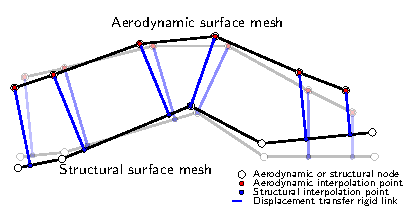
\includegraphics[width=0.5\textwidth]{images/rlink_displaced}
  \label{fig:rigid-link-displacement}}
  \subfloat[Load transfer rigid links]{
    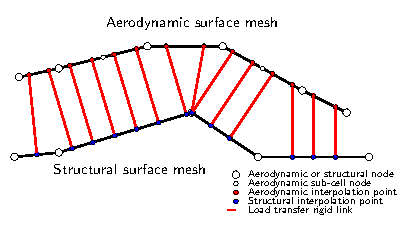
\includegraphics[width=0.5\textwidth]{images/rlink_displacement}
    \label{fig:rigid-link-force}}
  \caption{Load and displacement transfer rigid links for a
    second-order finite-element mesh.}
\end{figure}

For this project, our team will develop a coupled aeroelastic design
capability between TACS and $\text{SU}^2$, using existing parallel
load and displacement transfer
methods~\cite{Kennedy:2014:tacs-tripan}. The load and displacement
transfer technique in TACS are based on the method of virtual
work. The technique extrapolates the displacements from the structural
surface to the aerodynamic surface using both a series of rigid
links. These rigid links are constructed by finding the closest
structural surface point to each aerodynamic mesh location. The rigid
links for displacement extrapolation are illustrated in
Figure~\ref{fig:rigid-link-displacement}.

The aerodynamic surface loads are transferred from the aerodynamic
surface mesh to the structures using a consistent and conservative
technique, again based on rigid-link extrapolation.  The consistent
force vector is computed by performing an integration over the
deformed aerodynamic surface as follows:
\begin{equation}
  \begin{aligned}
    \delta\, W & = q \int_{S_{A}} \, C_{p} \, \hat{\mb{n}}^{T} \delta\mb{u}_{A} \, \mathrm{d}S \\
    & = q\int_{S_{A}} \, C_{p} \left( \hat{\mb{n}}^{T} \delta \mathbf{u}_{S} -
    \left( \hat{\mb{n}}\times \mb{r}_{SA} \right)^{T} \delta \mbs{\theta}_{S} \right) \, \mathrm{d}S,
  \end{aligned}
  \label{eqn:method-virtual-work}
\end{equation}
where $q$ is the dynamic pressure, $C_{p}$ is the surface pressure
coefficient $\mb{u}_{A}$ and $\mb{u}_{S}$ are the displacements at the
aerodynamic and structural surfaces, $\mbs{\theta}_{S}$ is the
rotation at the structural surface, $\mb{r}_{SA}$ is the rigid-link,
and $\hat{\mb{n}}$ is the normal defined on the deformed aerodynamic
surface.

The integral~\eqref{eqn:method-virtual-work} is approximated by
summing the contributions from each aerodynamic surface cell using a
two-part numerical quadrature rule. First, we split the aerodynamic
cells based on a specified characteristic length scale into a series
of sub-cells. The characteristic length scale is selected to match the
length scale of the average finite-element within the structural
model. If any cell-side exceeds the characteristic length scale, we
split the cell. Next, on each sub-cell we use a quadrature scheme that
matches the order of accuracy required by the underlying
finite-elements. For each quadrature point within each sub-cell, we
compute a rigid link from the quadrature point to the structural
surface in an analogous manner to the displacement transfer
scheme. This two-level quadrature rule is effective at smoothly
transferring loads to the finite-element mesh even in the presence of
high-aspect-ratio surface cells. Figure~\ref{fig:rigid-link-force}
illustrates the load transfer scheme including sub-cell refinement.

An important feature of the load and displacement transfer technique
implemented in TACS is that it accounts for nonlinear following
forces.  It is important to properly account for these forces when
analyzing very flexible structures subject to aerodynamic loads. In
addition, these following force terms are correctly linearized,
resulting in fast analysis and accurate derivatives for design
optimization.

\subsubsection{Low-fidelity aeroelastic framework}

A key element of this work will be a multi-fidelity framework that
includes aeroelastic and dynamic constraints on the aircraft.  These
constraints are especially important for flexible light-weight
aircraft.  To assess the dynamic aeroelastic characteristics of the
aircraft, we will use the existing capabilities of TACS coupled to the
low-fidelity aerodynamic panel code
TriPan~\cite{Kennedy:2014:tacs-tripan}. TriPan is a parallel,
unstructured three-dimensional panel code for calculating the
aerodynamic forces and moments for inviscid, external lifting flows
governed by the Prandtl--Glauert equation, and has been used for a
number of static and dynamic aeroelastic design optimization
studies~\cite{Kennedy:2014:tacs-tripan, Kennedy:2012:CMC,
  Kennedy:2013:SDM, Kennedy:2014:High-aspect-ratio,
  Kennedy:2014:Aviation}. A benefit of using TACS and TriPan is that
it will provide a fast and robust tool for early design space
exploration. While the existing TACS/TriPan tool will be used within
the project, our objective remains to integrate and use the
multi-fidelity aeroelastic design optimization tools for all aspects
of the design.


    % \subsection{Structural Dynamics Modeling (Glenn/AeroVelo)}

    % Structual dynamics are a very important design consideration for aircraft with highly flexible wings. Large spans and low mass
    % combine to make dynamic bending modes and structural response to control inputs both key constraining factors. NASA's Helios 
    % aircraft experienced a catastrophic failure related to unexpected structural dynamic response, clearly demonstrating the importance
    % of accouting for this phenomenon in these types of aircraft. 
    % However, directly modeling it with high fidelity codes is currently computationally infeasible in an optimization context. Never the less, 
    % some analysis needs to be included in the system model to account for these issues. Mark Drela's ASwing code is a lower fidelity 
    % coupled aero-structural analysis tool that can account for the non linear structural dynamics using a beam based method\cite{DrelaASWING}. This tool was specifically built for this type of application to be used in a rapid iteration design process. It  
    % will be coupled in to the overall system model. 

    % Although ASwing does not provide analytic derivatives, its low computational cost makes it feasible to use finite difference to 
    % get the disciplinary derivatives. These can then be combined with the other disciplines by OpenMDAO's mixed derivatives capabilities
    % to maintain the high efficiency of the overall design optimization. 

    \subsection{Aircraft Design}

        AeroVelo will be responsible for the actual design of the human powered aircraft. They will complete a conceptual design 
        phase early on in the effort to determine the major configuration level aspects of the aircraft such as wing span, pilot pod
        locations, propeller placement, and wing construction methods. At the end of this design phase, a summary report detailing
        the analyses done and the design decisions made from the data generated will be written. 

        \subsubsection{Aircraft Configuration}

        The Keremer Marathon Challenge demands a very high speed for a human powered aircraft over an extended period of time. To reach the 
        required speeds, the power aircraft will require on the order of 1 KiloWatt of continuous power. This power output is not 
        sustainable by a single pilot for the length of time needed to complete the challenge, so AeroVelo has proposed using multiple 
        pilots to lower the per-pilot power requirements. Their current concept uses 3 pilots, located in separate pods spaced out 
        span-wise along the wing. This lowers the per-pilot power requirements considerably, and also introduces a unique loading profile 
        for the wings. 

        In order to complete the conceptual design phase, AeroVelo will rely heavily on existing low-fidelity analyses for aerodynamic and 
        structural modeling. They will build these models into an initial system model of the aircraft inside the OpenMDAO framework. 
        This initial model will guide the conceptual design process and also provide a baseline to integrate the higher fidelity models into. 
        OpenMDAO provides a key benefit for this work, because it allows the team to build a flexible and modular system model where fidelity can 
        be increased as better models are made available. 

        \subsubsection{Construction Methods}

        There are two relevant construction methods that have been applied on these types of aircraft in the past. The MIT Deadalus, 
        AeroVelo Atlas, and the AeroVironment HELIOS both used a somewhat traditional spar-rib construction method. The spars are 
        made from long carbon-fiber tubes, and the ribs are made from and balsa wood or composites. The skin is built from a
        combination of thin mylar and foam. The foam is used on the upper surface and leading edge to help retain the correct airfoil 
        shape necessary to achieve laminar flow. In his construction method, the spar carries almost all of the bending and torsional 
        loads for the wing, and the skin does not contribute any significant stiffness. Figure~\ref{fig:traditional-wing-construction} shows
        details the Deadalus style wing construction method. 

        \begin{figure}[!hbt]
                \centering
                % 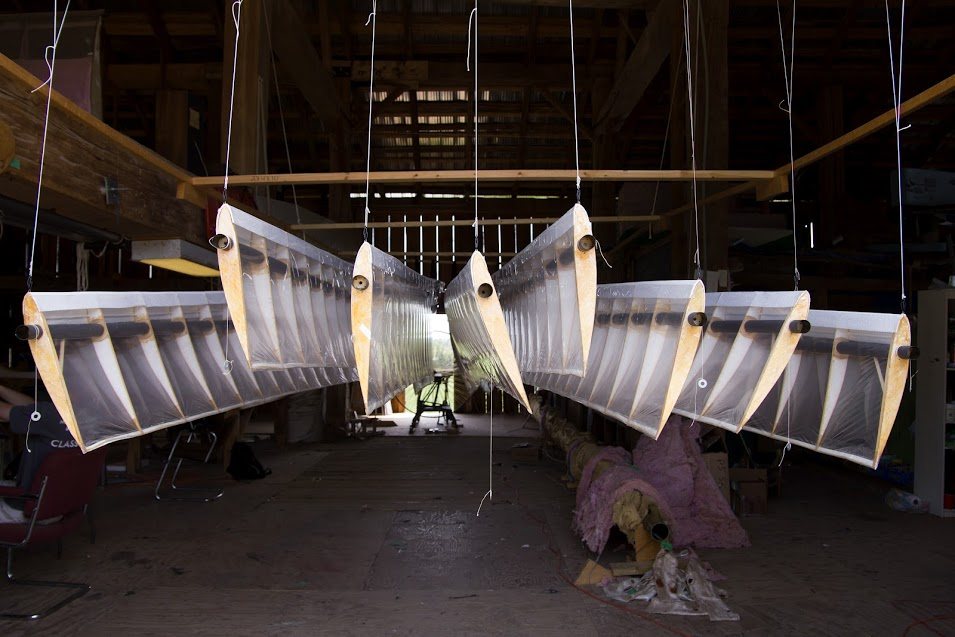
\includegraphics[width=.75\textwidth]{images/wing-construction}
                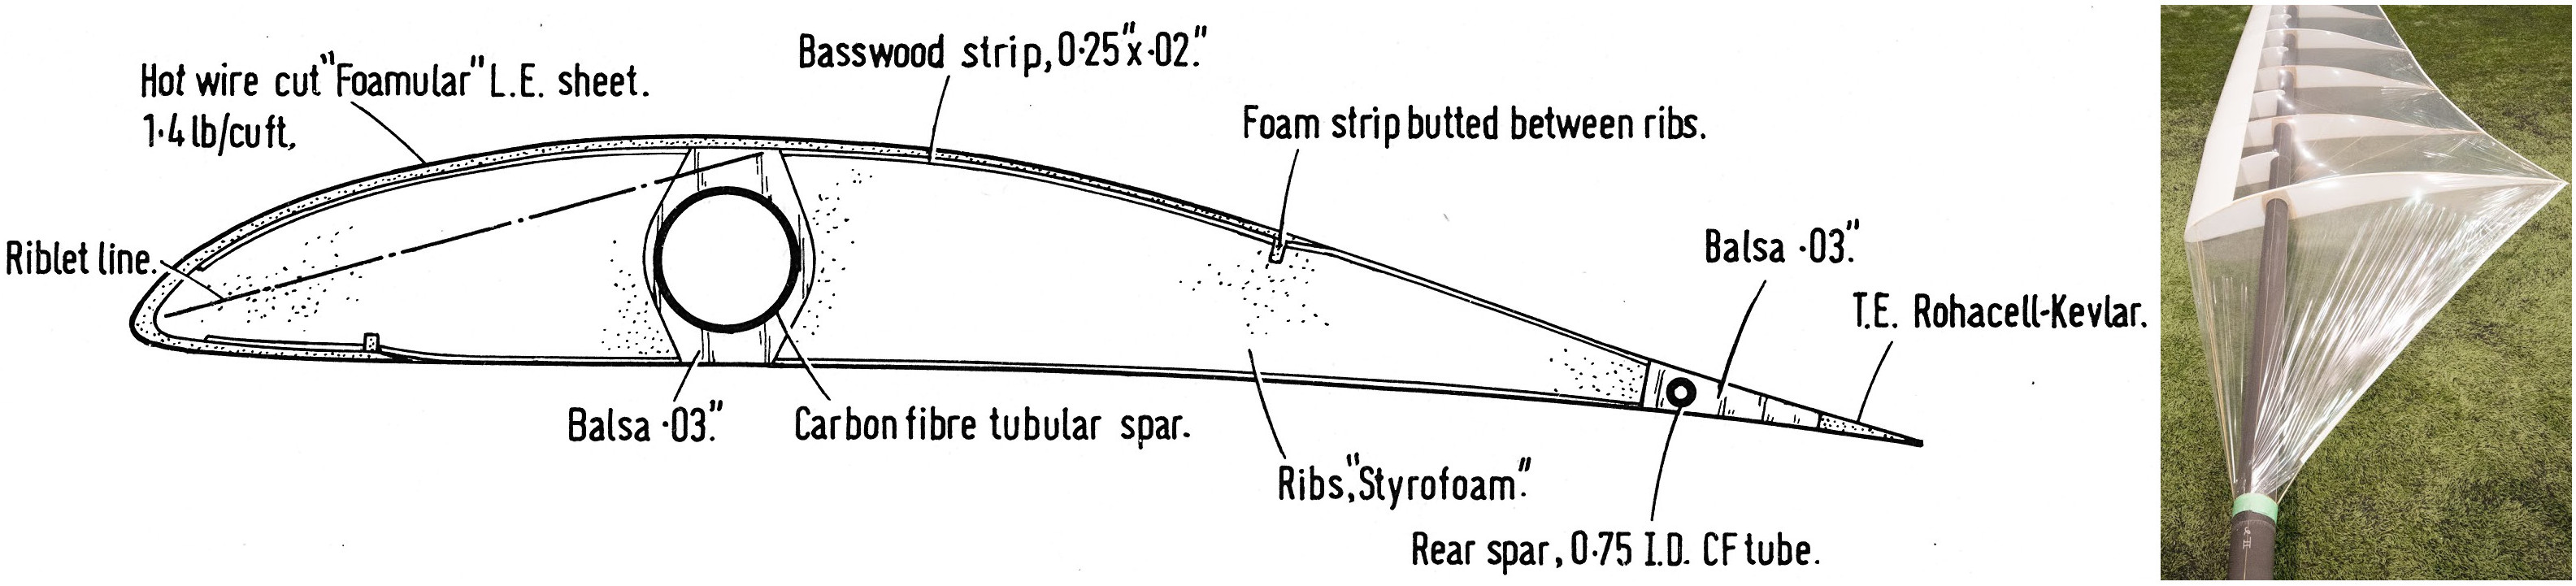
\includegraphics[width=.9\textwidth]{images/traditional-wing-construction}
                \caption{Left: A cross sectional diagram of the Daedalus wing construction method, highlighting the leading edge foam sheeting
                and round carbon fiber main spar. Right: Actual Atlas helicopter rotor blade using this construction method.}
                \label{fig:traditional-wing-construction}
        \end{figure}

        But a recent, highly successful, human powered aircraft called the Musculair 2 used a stressed skin construction
        method. This aircraft used a full carbon fiber skin combined with a carbon fiber I-beam for their wing seen in 
        Fig.~\ref{fig:musculair-wing-construction}. Using this construction method, the I-beam carries the bending loads, 
        while the skin handles most of the bending loads. The primary motivation for using this new method was to achieve 
        a more consistent as-flow airfoil shape allowing them to achieve more laminar flow and lower overall drag. Although 
        this method is better aerodynamically, it is also heavier than the spar and rib based method. 

        \begin{figure}[!hbt]
                \centering
                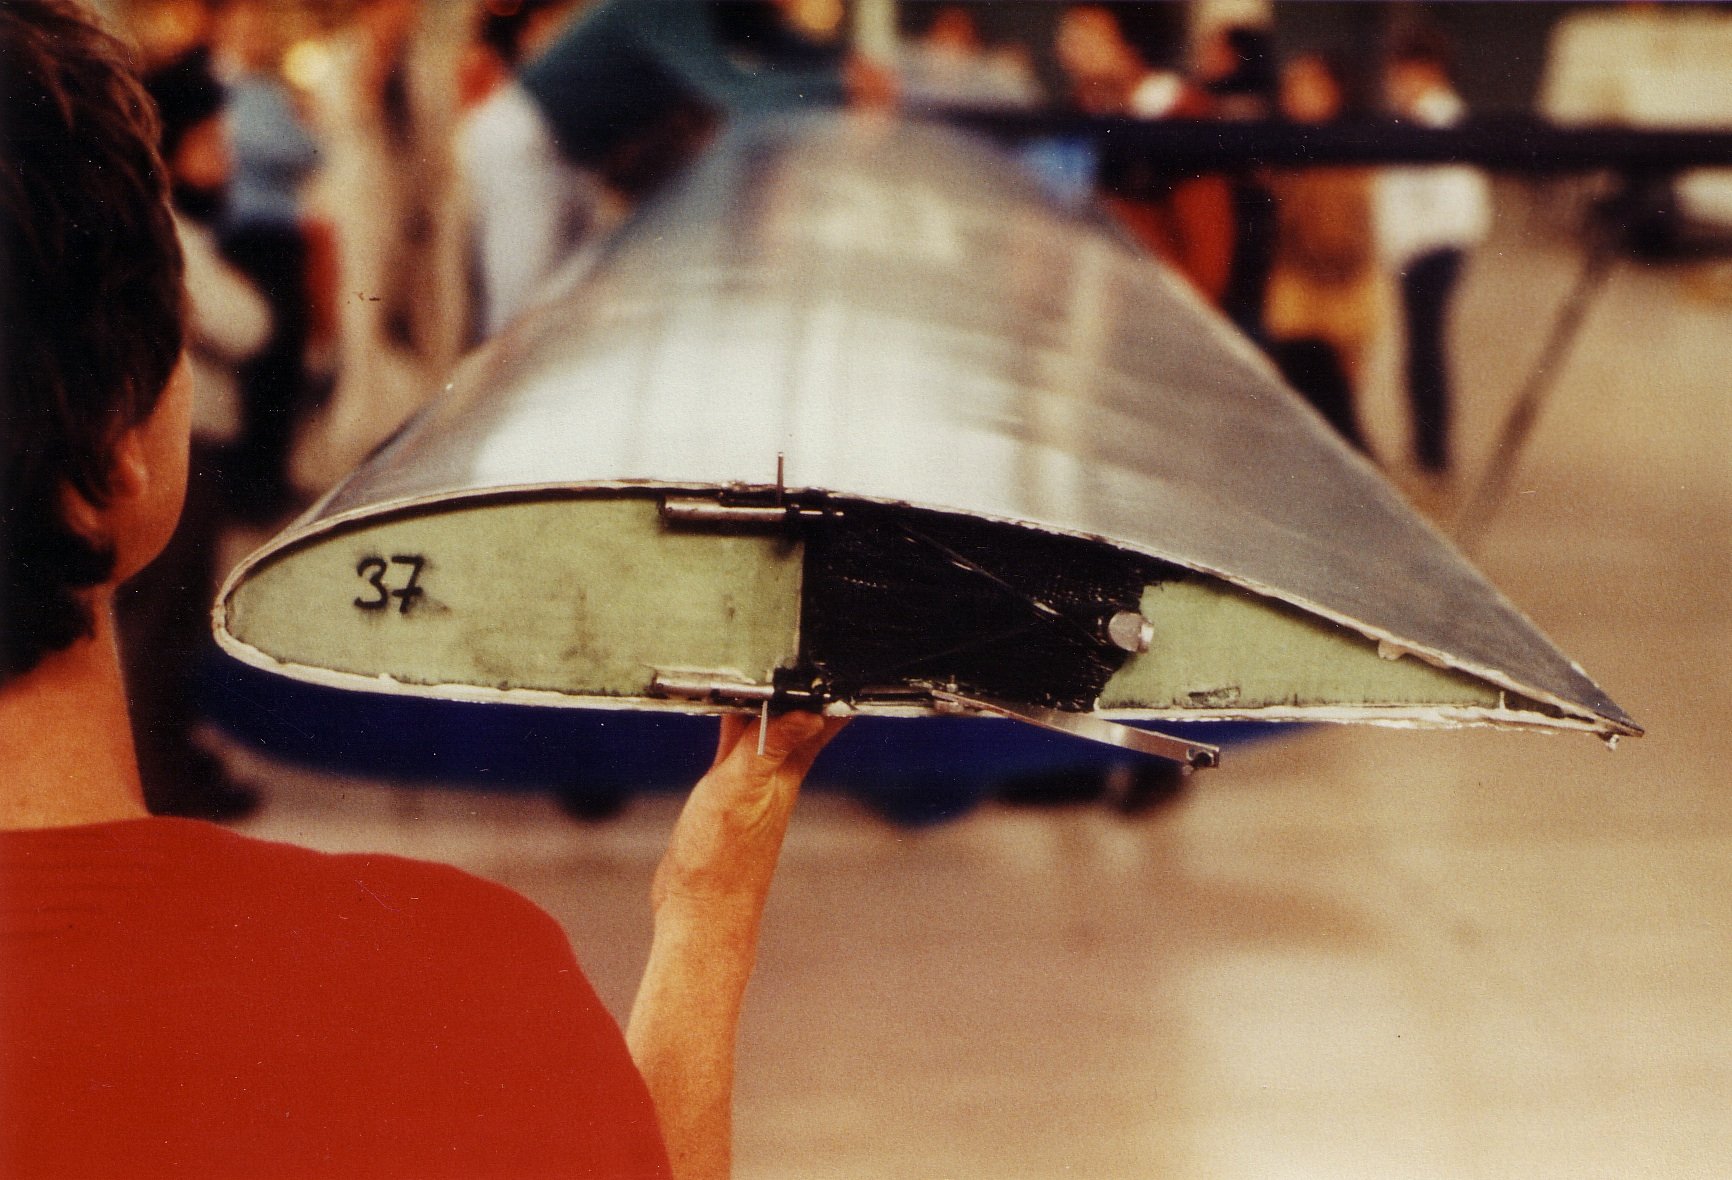
\includegraphics[width=.75\textwidth]{images/musculair2-wing-construction}
                \caption{Wing construction for the Musculair 2 aircraft, utilizing a stressed carbon fiber skin and I-beam 
                to handle bending and twisting loads.}
                \label{fig:musculair-wing-construction}
        \end{figure}

        AeroVelo be selecting between these two construction methods as part of the conceptual design process. They will use 
        OpenMDAO to build an Aero-elastic model that will allow them to understand the trade between aerodynamics and weight 
        that is fundamental to selecting between the two construction methods. 

        \subsubsection{Detailed Design}

        After the conceptual design phase is complete, AeroVelo will perform a complete detailed design of the aircraft. This 
        design phase will rely heavily on the high-fidelity aero-propulsive elastic models built by the other team members. 
        These models will be used to finalize the propeller sizing, aerodynamic shape, and structural design of the aircraft. They will pick 
        between three possible drive trains: chain and sprocket, gear and shaft, or all electric. All other details (e.g. control
        surface sizing and location, pilot positioning, landing gear, etc.) will also be defined to complete the aircraft 
        design. 

        A the end of this design phase, a detailed design report will be written that captures all of the analyses done 
        and the data that was generated. The decisions made about the design will be documented along with the key data that 
        supported those decisions. The report will include a detailed geometry model of the whole airplane. 



    \subsection{Structural Testing \& Model Validation}
        
        Highly flexible wing structures, which yield very large deflections, demand the use of non-linear structural models. 
        Application of these non-linear models in a aero-propulsive-elastic optimization context is one of the major innovations of this 
        work. Due to it's novel application, these models are also one of the largest sources of uncertainty in the analysis models. 
        To help mitigate this uncertainty, it is necessary to perform some destructive structural testing of of structures undergoing large 
        deflections. This testing will be performed on test articles built by AeroVelo Inc. Data will be collected using 
        NASA Armstrong's Compact Fiber Optic Sensing System (CFOSS). CFOSS offers several important features that will make the 
        data collected of high value for tool validation purposes and also make it uniquely qualified to be applied to human powered vehicles. 

        \begin{figure}[!hbt]
            \centering
            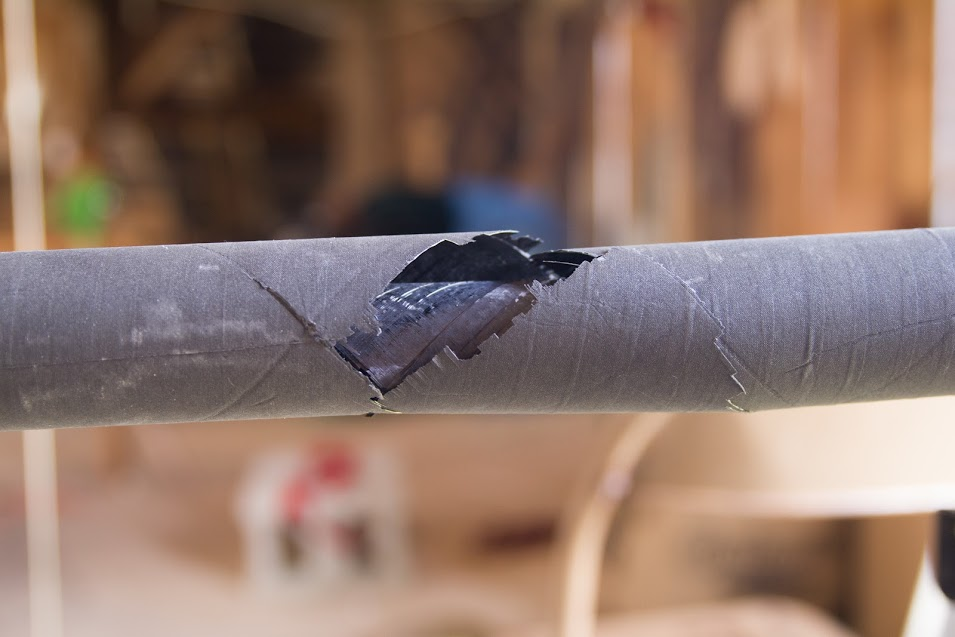
\includegraphics[width=.5\textwidth]{images/spar_failure}
            \caption{A strain induced spar failure from structural testing for the AeroVelo Atlas human powered helicopter.}
            \label{fig:spar-failure}
        \end{figure}

        First, CFOSS offers a very high resolution for measurements. This will be key in collecting high quality data for the validation 
        of the TACS predictions. In the types of ultra-light structures that are built for these aircraft, the structural failure can 
        occur anywhere along the length of the wing spar, as seen in Fig.~\ref{fig:spar-failure}. By using the 
        high resolution of the CFOSS system, the data will capture the detailed loads across the entire structure 
        which can then be matched up with the predicted results and the models can be adapted to more accurately 
        predict the response of the structural models.

        Second, CFOSS is an extremely lightweight system, designed to be used for real time structural health monitoring applications.
        It is much lighter and smaller than traditional strain gage based system. Given the extreme sensitivity to weight
        that human powered aircraft (or any super lightweight aircraft) has, the CFOSS technology is critical to enable its usage during 
        flight testing and eventually normal operations. 


        \begin{figure}[!hbt]
            \centering
            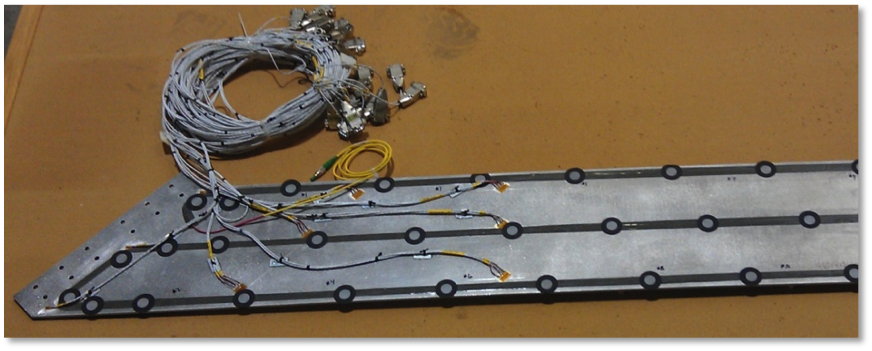
\includegraphics[width=.9\textwidth]{images/cfoss_vs_straingauge}
            \caption{The cfoss system embedded on this test article is significantly smaller and lighter than the strain gage system, 
            despite having an 30 times as many sensors. }
            \label{fig:cfoss-vs-straingauge}
        \end{figure}


        \subsection{Testing Plan}

        AeroVelo will produce a 10 meter long spar to be used as a test article and will perform the structural testing 
        at their own facilities, using existing testing rigs. The testing has 
        two distinct goals. Firstly, it will generate validation data to confirm the predictions 
        of the non-linear structural modeling methods being used in TACS. Secondly, it will provide AeroVelo with a mechanism 
        to validate the as-built strength of their spars. The as-built strength of the spar is a function of the materials used 
        in its construction as well as the construction methods themselves. To keep weight to its absolute minimum, 
        its important to have an accurate estimate for strength to avoid the need for excessive structural margins. 

        \begin{figure}
            \centering
            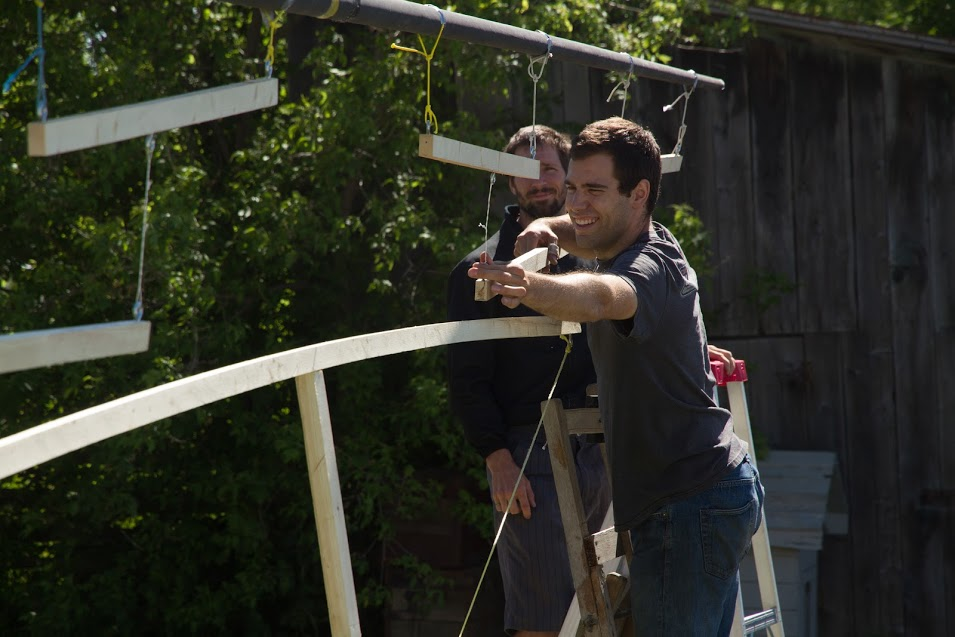
\includegraphics[width=.5\textwidth]{images/structural_test}
            \caption{Todd Reichert and Cameron Roberston testing a wing spar for the Atlas Human Powered Helicopter using a
            jig to get distributed loading. }
            \label{fig:spar-load-test}
        \end{figure}

        In previous efforts, AeroVelo has used a distributed dead weight approach for loading their spars during testing. 
        Figure~\ref{fig:spar-load-test} shows the setup AeroVelo used to get a distributed load applied to the spar. 
        For this effort, a different loading mechanism is needed. Using a dead load applies a purely downward force to the 
        structure, which is a reasonable approximation when the deflections are small. However, the aerodynamic loads will 
        be applied normal to the structure in reality, and for large deflections the surface normal vector will not be 
        close to vertical anymore. 

        \begin{figure}[!htbp]
            \centering
            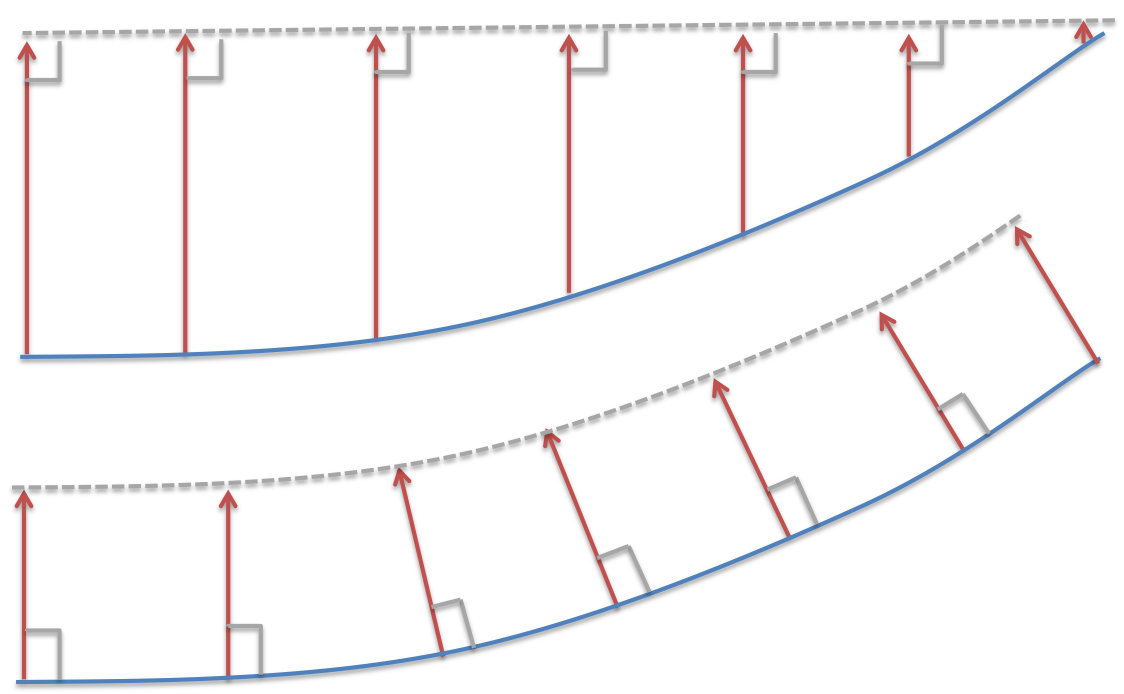
\includegraphics[width=.75\textwidth]{images/follower_force}
            \caption{The upper diagram shows loads applied in a single direction, as demonstrated in Fig.~\ref{fig:spar-load-test}. However, loads applied normal to the surface, as shown in the lower diagram, are important for accurate testing of structures with large deflections.}
            \label{fig:follower-force}
        \end{figure}

        So the testing will be conducted using a loading mechanism that applies appropriate loads in the normal direction
        as the spar deflects, as illustrated by the lower diagram in Fig.~\ref{fig:follower-force}. Data will be collected, using CFOSS, for pure bending and bend-twist loads for a series of different 
        load levels. After a series of non-destructive tests are preformed to generate stress and strain validation data, the test 
        article will go through a set of destructive tests to generate ultimate strength data. 


  \section{Innovation \& Impact}

    \subsection{Kremer Prize}
    The Kremer marathon challenge was established in 1959, and has remained unmet for the last 55 years. 
    Successful completion of work proposed here could result in could result in finally achieving this very challenging
    aviation milestone. AeroVelo is already well know for their 2013 claiming of the Sikorski Prize with their Atlas 
    Human Powered Helicopter. Their stated mission is ``to inspire the public and youth, tackle the impossible, and 
    challenge conventional design by doing more with less.'' Partnering with AeroVelo for this work will bring a significant
    amount of visibility to the results of this work and help raise awareness of the public benefit from NASA's advanced 
    multidisciplinary design research. 

    \subsection{Validation of Advanced Simulation Methods}
    Additionally, the work will significantly advance state-of-the art for design methods of highly flexible wings. 
    A fully coupled high-fidelity nonlinear structural, aerodynamic modeling method will represent a significant advancement 
    in capability. By also including propeller effects on the aerodynamics of the wing, we will be demonstrating an even larger 
    degree of multidisciplinary coupling. Furthermore we will be demonstrating 
    how gradient based optimization, with analytic gradients, methods can be applied to this new class of aircraft design problems 
    to dramatically improve the design process.

    Furthermore, the integration of multidisciplinary design optimization into an actual aircraft design process represents
    a tremendous opportunity to learn how it can be used more effectively in a design context. By combining optimization, 
    testing, and actual flight into a single effort we gain the opportunity to iterate not just on the aircraft 
    design but also on the design process itself. We'll be able to improve the usefulness of optimization tools by 
    tailoring them to support a iterative design loop. So the work proposed here will yield a large amount 
    of information on how to better integrate multidisciplinary methods into the aerospace community at large. 

    \subsection{Commercial Applicability}
    Beyond increased academic understanding, the tools would be designed to easily translate into commercially beneficial
    modeling capabilities. The advancement of long endurance unmanned aerial vehicles (UAVs) requires new designs
    and simulation toolsets that push the envelope in terms of structural weight and power requirements. 
    This new class of high-altitude long-endurance (HALE) aircraft are the subject of commercial,
    military and scientific interest, from companies including QinetiQ, Titan Aerospace, General Atomics, Scaled Composites, and Boeing, 
    Facebook, and Google. 

  
\section{Intellectual Property Statement}
    All designs and models developed under this effort will be released under the Apache V2.0 Open Source License. The intention 
    of the team is to provide the widest possible dissemination of all the knowledge and data data. The open source license helps 
    ensure broad availability of the information to the public. 

    A github repository will be set up to host all the information. This repository will serve as the collaboration 
    hub for the research team during the effort as well as mechanism for public dissemination of the results. 

\section{Team Structure and Management}
    Justin Gray, from NASA Glenn Research Center, will be the principal investigator for this work. Justin will also perform 
    project management duties, and serve as the interface to NARI for all reporting efforts. NASA Glenn will be the lead 
    center for this effort, serving to orchestrate and organize the efforts of the other team members. 

    The NASA team members come from three different NASA Centers: Glenn, Ames, and Armstrong. The other team members come from three different external organizations. Table~\ref{tab:team-expertise} summarizes the team members and their expertise. In order to facilitate the 
    collaboration, monthly virtual meetings will be held with the whole team. These meetings will allow progress updates and coordination 
    between all members. In addition, an in person meeting will be held within the first 3 months of the effort to serve as a design workshop 
    led by AeroVelo where the team will all go review the conceptual design of the aircraft and work to establish the proper baselines 
    for all their models. 

    The structural testing, conducted at AeroVelo facilities, will involve a coordinated effort between AeroVelo, NASA Glenn, 
    NASA Armstrong, and the Georgia Institute of Technology. These tests are expected to take about 1 week, and team members 
    from AeroVelo, NASA, and the Georgia Institute of Technology will attend to help conduct the experiments and collect the data. 

    \begin{table}[htb!]
        \caption{NASA team member names, centers, and responsibilities}
        \centering
        \begin{tabular}{lll}
            \textbf{Team member}  & \textbf{Organization} & \textbf{Expertise} \\ \hline
            Justin Gray & NASA Glenn & \bigcell{l}{Propulsion systems analysis, \\ multidisciplinary optimization} \\
            Jeff Chin & NASA Glenn & \bigcell{l}{Propulsion systems analysis, \\ engine dynamics and controls}  \\ 
            Kevin Reynolds & NASA Ames & \bigcell{l}{Aero-propulsive-servo-elastic aircraft design, \\ autonomous aircraft design}  \\
            Anthony Piazza &  NASA Armstrong  & CFOSS installation and data collection \\
            Dr. Graeme Kennedy & \bigcell{l}{Georgia Institute \\ of Technology} & \bigcell{l}{Aerostructrual optimization, \\ composite structures} \\
            Dr. Juan Alonso & Stanford & \bigcell{l}{Aerodynamic Shape Optimization, \\ Aircraft Design} \\
            Aero Velo Team & Aero Velo Inc & \bigcell{l}{Human powered aircraft experts \\ composite structures construction}\\
        \end{tabular}
        \label{tab:team-expertise}
    \end{table}


\begin{landscape}
\section{Milestones and Deliverables}
    \subsection{Schedule}
        \begin{figure}
            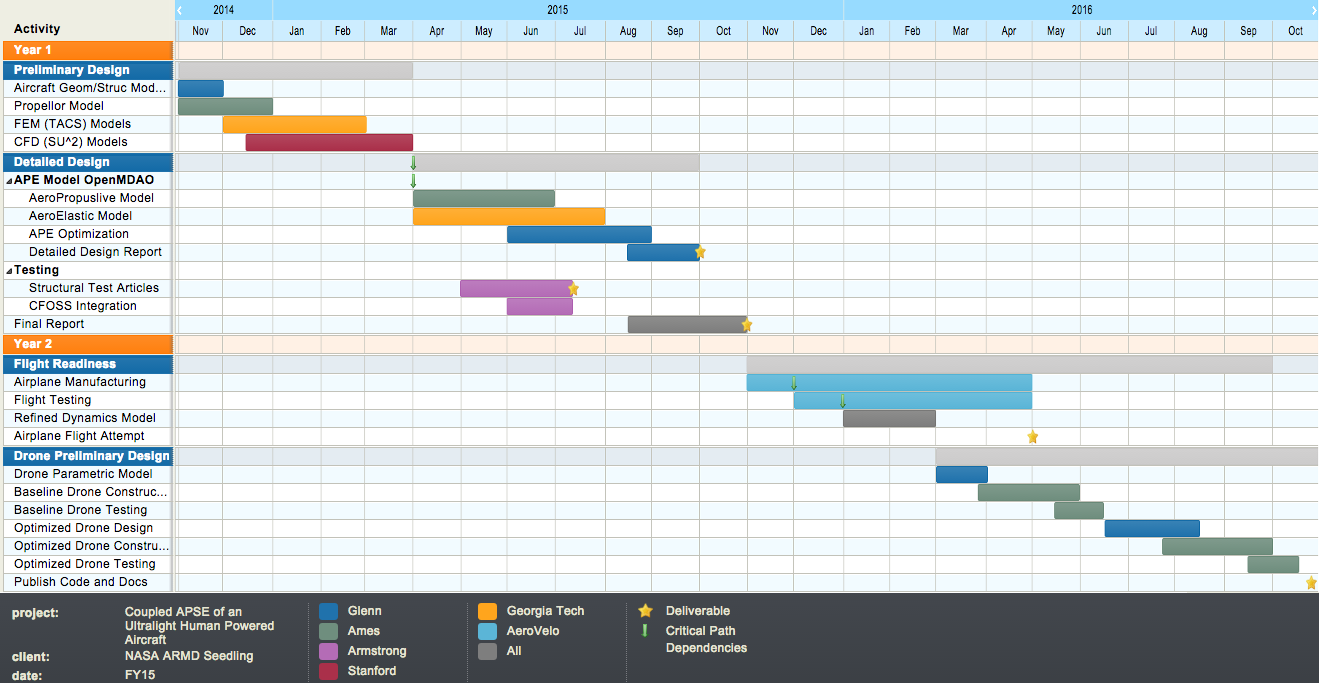
\includegraphics[width=\hsize]{images/gantt_v2}
        \end{figure}
 \end{landscape}
    \subsection{Milestones}
        \begin{table}\begin{tabular}{lcl}
            \textbf{Milestone}          & \textbf{Due Date} & \textbf{Exit Criteria} \\ \hline
            \textit{ \textbf{Year 1}} & \\
            Aircraft Geometry           & 11/30/2014 & Parametric geometry/structural model  \\
            Propeller Geometry          & 12/30/2014 & Parametric geometry model for the propeller \\
            FEM Model                   & 2/30/2015 & FEM Mesh model of aircraft structures \\
            CFD Model                   & 3/30/2015 & Unstructured Volume Mesh of the Wing \\
            Preliminary Design           & 3/30/2015 & Conceptual design report for Marathon Aircraft  \\
            Aero-Propulsive Analysis    & 6/30/2015 & OpenMDAO model with propeller coupled to CFD \\
            Structural Testing          & 7/15/2015 & Complete structural test report \\
            Aero-Elastic Analysis    & 7/30/2015 & OpenMDAO model with aero coupled to structures \\
            \bigcell{l}{Aero-Propulsive-Elastic \\ Optimization} & 8/30/2015 & Completed optimization of vehicle \\
            Detailed Design             & 9/30/2015 & Detailed design report for Marathon Airplane \\
            \textit{ \textbf{Year 2}} & \\
            Refined APE Model           & 2/30/2016 & Refined and adapted model based on construction \\
            Drone Parametric Model      & 3/30/2016 & Preliminary design of a baseline ultra-light drone configuration \\
            Marathon Flight Testing     & 4/30/2016 & Finalized marathon plane testing and flight readiness review \\
            Baseline Drone Construction & 5/30/2016 & Construction of the ultra-light baseline drone \\
            Baseline Drone Testing      & 6/15/2016 & Collecting flight performance data from the baseline design \\
            Optimized Drone Design      & 8/15/2016 & Finalized design for an APE optimized drone \\
            Optimized Drone Construction & 9/30/2016 & Construction of the optimized ultra-light drone \\
            Optimized Drone Testing     & 10/15/2016 & \bigcell{l}{Compare optimized drone performance against \\
                                           baseline, further model validation} \\
        \end{tabular}\end{table}

    \subsection{Deliverables}
        \subsubsection{Year 1}
            \begin{itemize}
                \item Structural Test Articles (AeroVelo)
                \item Aerodynamic Models (Stanford)
                \item Structural Models (GaTech)
                \item Integrated System Model in OpenMDAO (NASA Glenn/Ames)
                \item Final Report (All)
            \end{itemize}
        \subsubsection{Year 2}
            \begin{itemize}
                \item Structural Dynamics Models (Stanford/GaTech)
                \item CFOSS Integrated Spar (NASA Armstrong)
                \item Flight Test Plan (AeroVelo)
                \item Drone Comparison Report (NASA Ames)
                \item Published Code/Design/Docs (All)
            \end{itemize}


  \section{Cost Sharing}
    AeroVelo Inc. will be primarily responsible for all aircraft design and testing during this effort. 
    They have committed their own funds for this project, without any additional NASA funding being delivered.
    This makes their involvement in the effort completely self funded and highlights the high value they see 
    in collaborating with NASA on this effort work. Their estimated expenses for the first year of the project are \$200,000 
    which will cover two engineers salaries, as well as all expenses for the construction of the necessary 
    structural test articles and testing rigs. NASA will pay for the CFOSS system for data collection during the 
    structural testing, including the costs of the fiber optic cables and measurement controller system. The costs for 
    the CFOSS system will come to approximately \$40,000.


  % \section{Resource Planning}
  %   \subsection{Test Facilities}
  %   \subsection{Supercomputing Resources}
  %       The project will require access to the NAS Cluster, to be able to run the coupled high fidelity simulations. 
  %       100,000 Standard Billing Units will be needed in Phase 1 of the effort. 

  \clearpage
  \bibliography{references}

  \appendix
  \clearpage
  \centerline{\huge{\textbf{Appendix}}}

  \begin{landscape}
  \section{Budget}
    \centering
    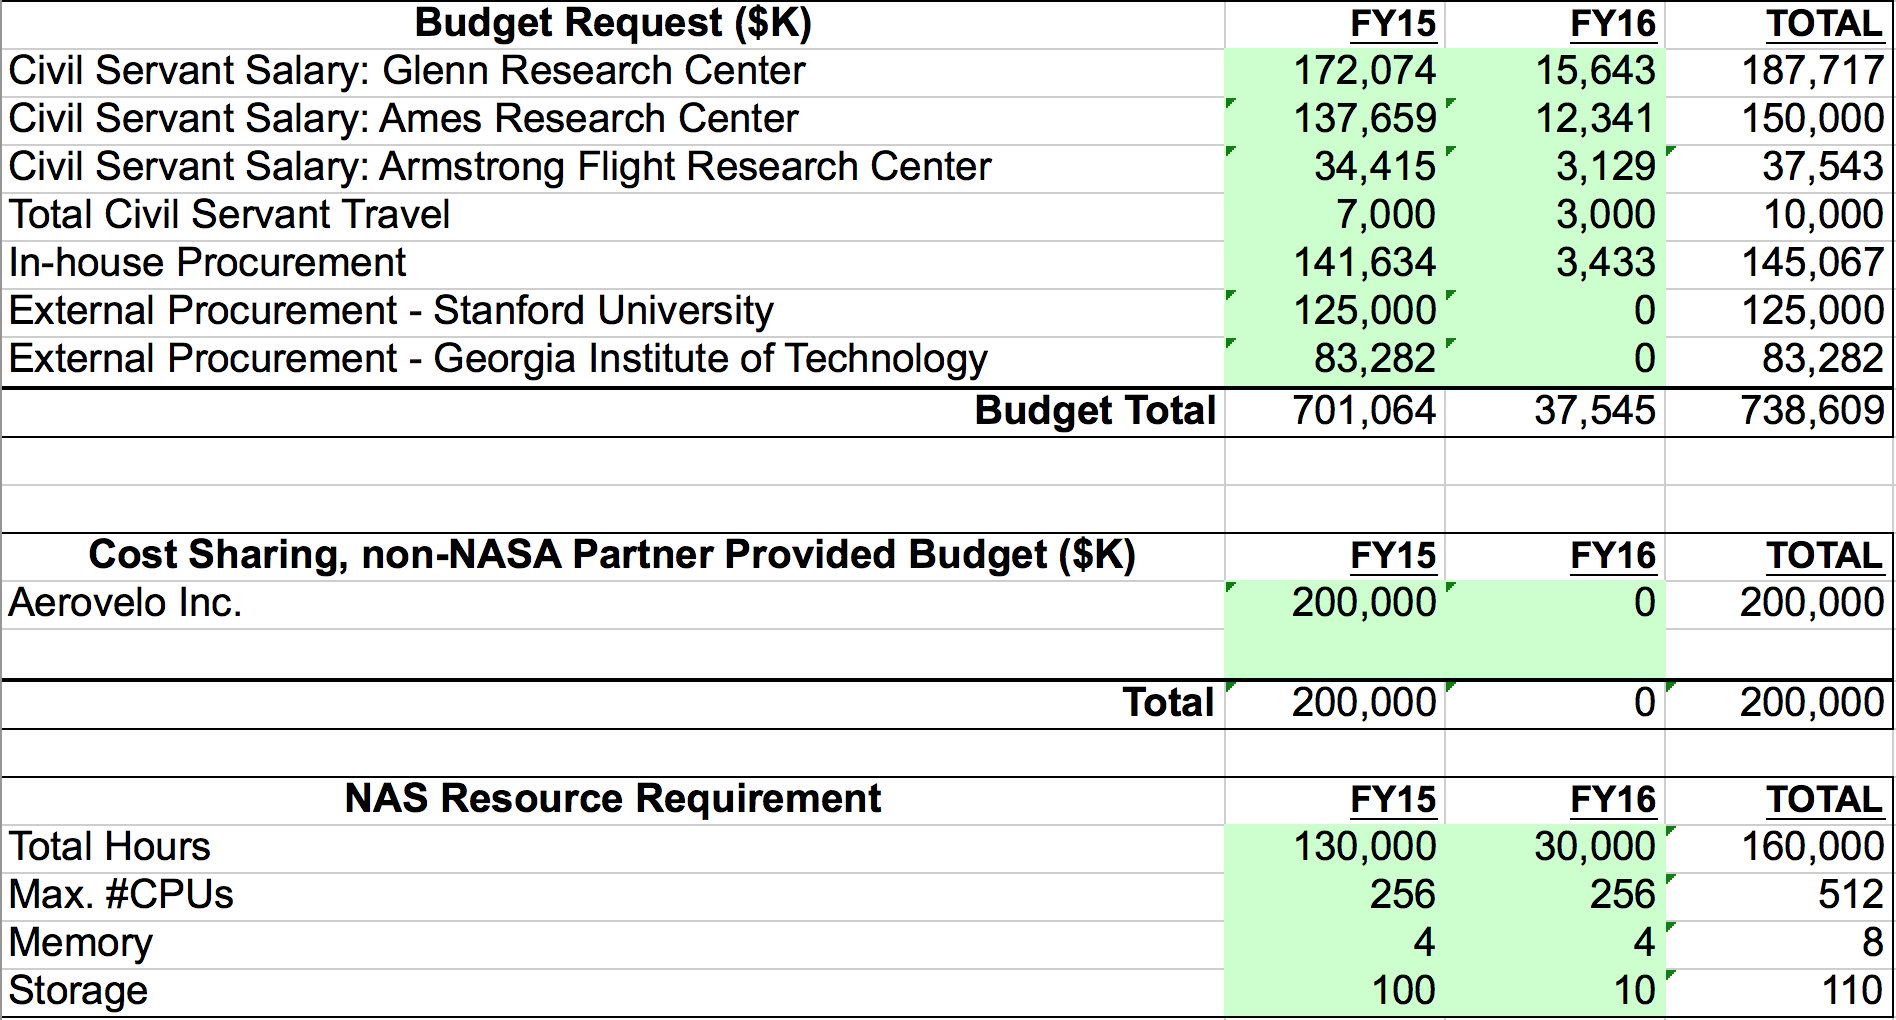
\includegraphics[height=\textheight]{images/budget_request}
    \end{landscape}

  \subsection{Stanford Itemized Budget}
    \begin{table}\begin{tabular}{l c}
    Graduate Student salary, tuition, and overhead &  \$80,000 \\
    Faculty Member (Juan J. Alonso), 3\% AY, 33\% Summer salary & \$41,250 \\
    Travel funds (for team meetings, necessary reviews, presentation of work at a conference) & \$3,750 \\
    \hline
    Total & \$125,000 \\ 
    \hline
    \end{tabular}\end{table}
  \subsection{Georgia Institute of Technology Itemized Budget}

    \begin{table}\begin{tabular}{l c}
    Graduate Student salary, tuition, and overhead &  \$60,000 \\
    Faculty Member (Juan J. Alonso), 3\% AY, 33\% Summer salary & \$20,250 \\
    Travel funds (for team meetings, necessary reviews, presentation of work at a conference) & \$4,750 \\
    \hline
    Total & \$85,000 \\ 
    \hline
    \end{tabular}\end{table}

  \clearpage

  \section{Letters of Collaboration}

    \newgeometry{left=0cm,bottom=0cm,top=0cm,right=0cm}
    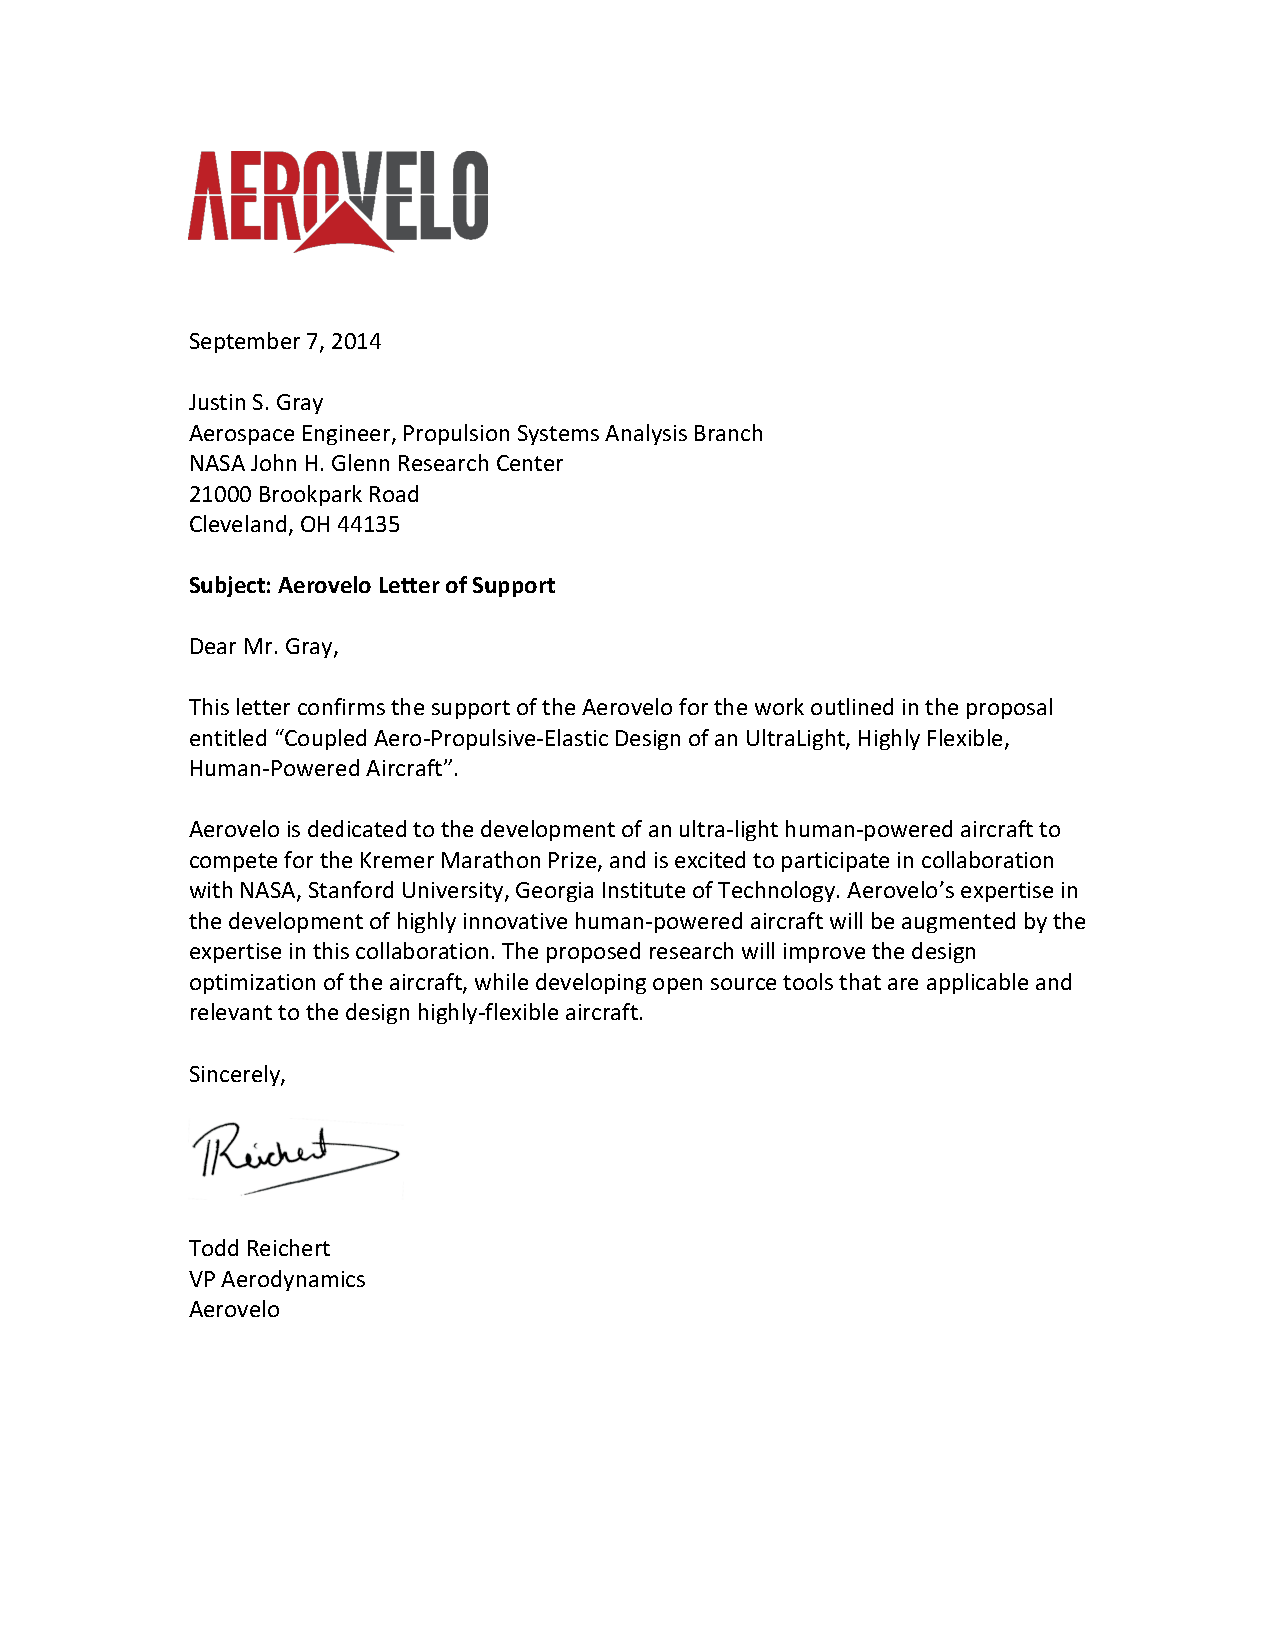
\includepdf[scale=1., pages={1}]{letters_of_commitment/aero_velo.pdf}
    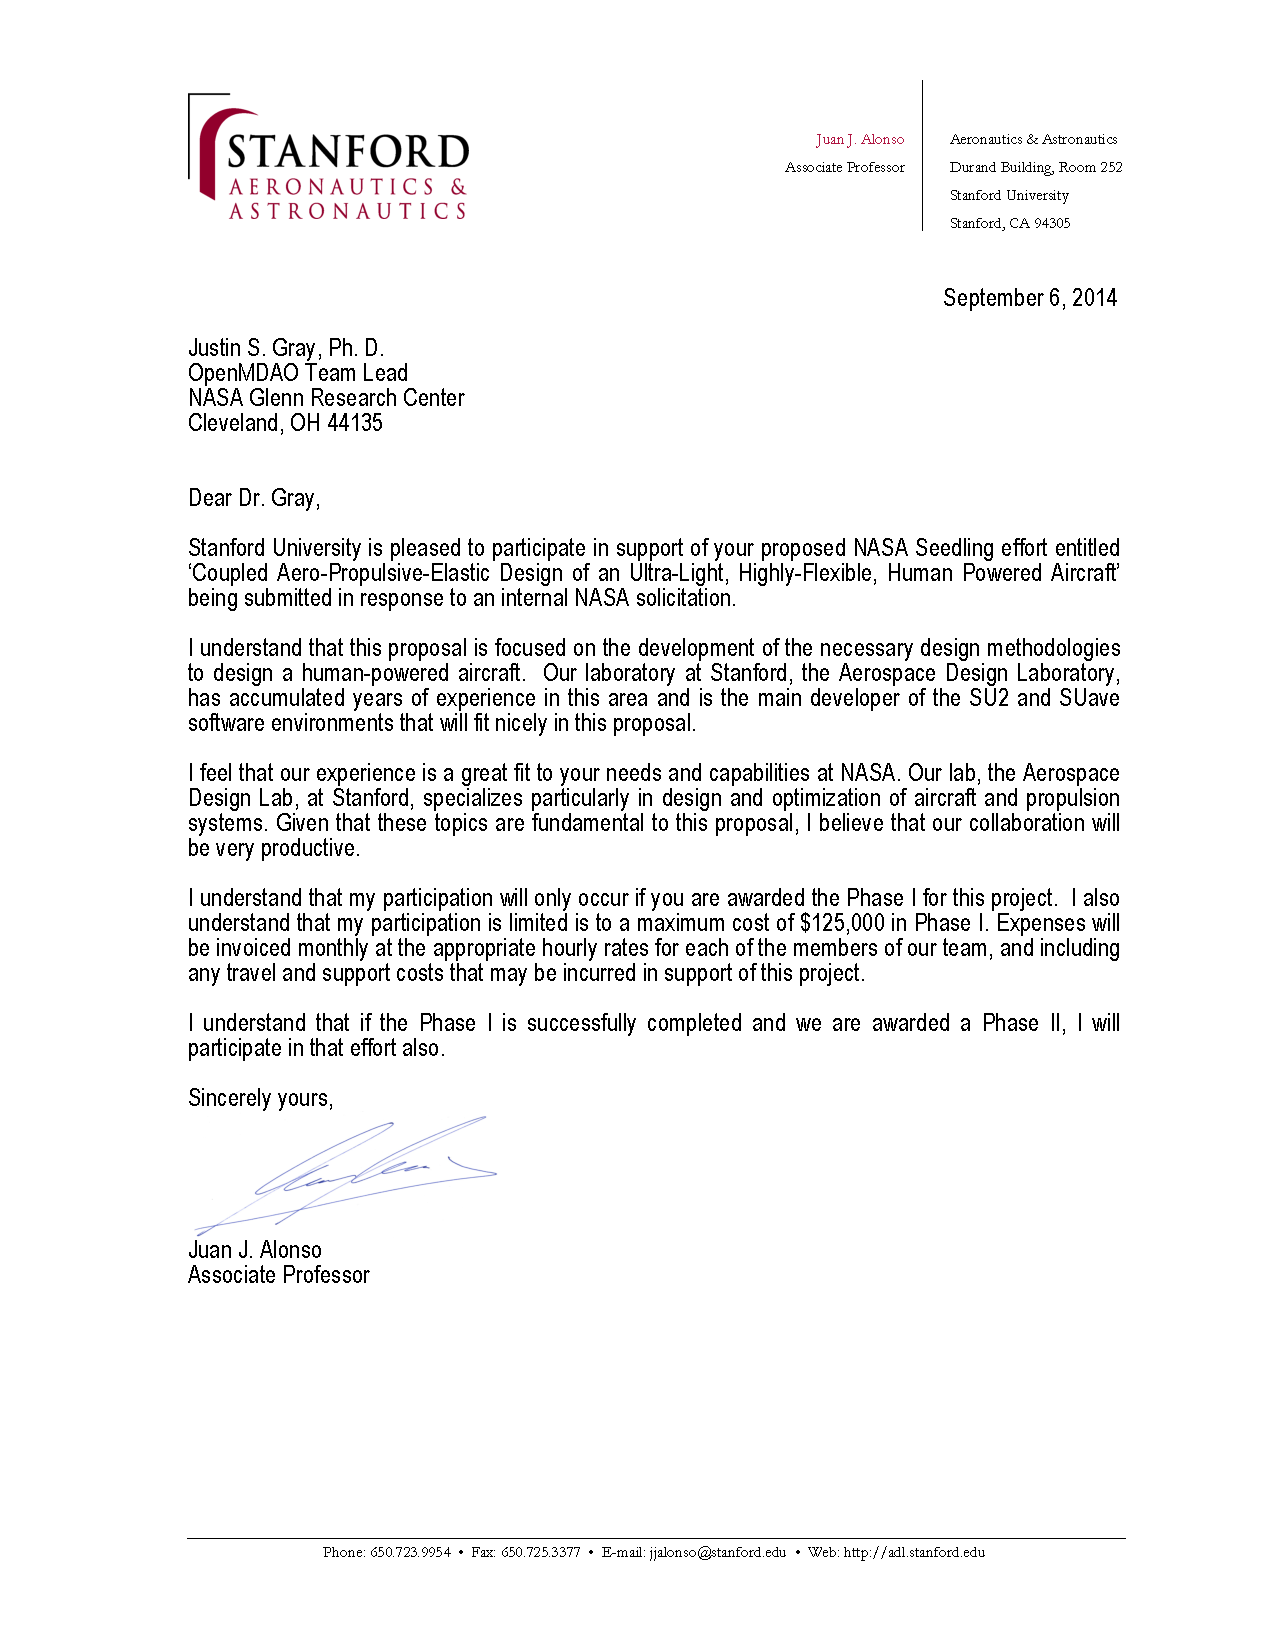
\includepdf[scale=1., pages={1}]{letters_of_commitment/stanford.pdf}
    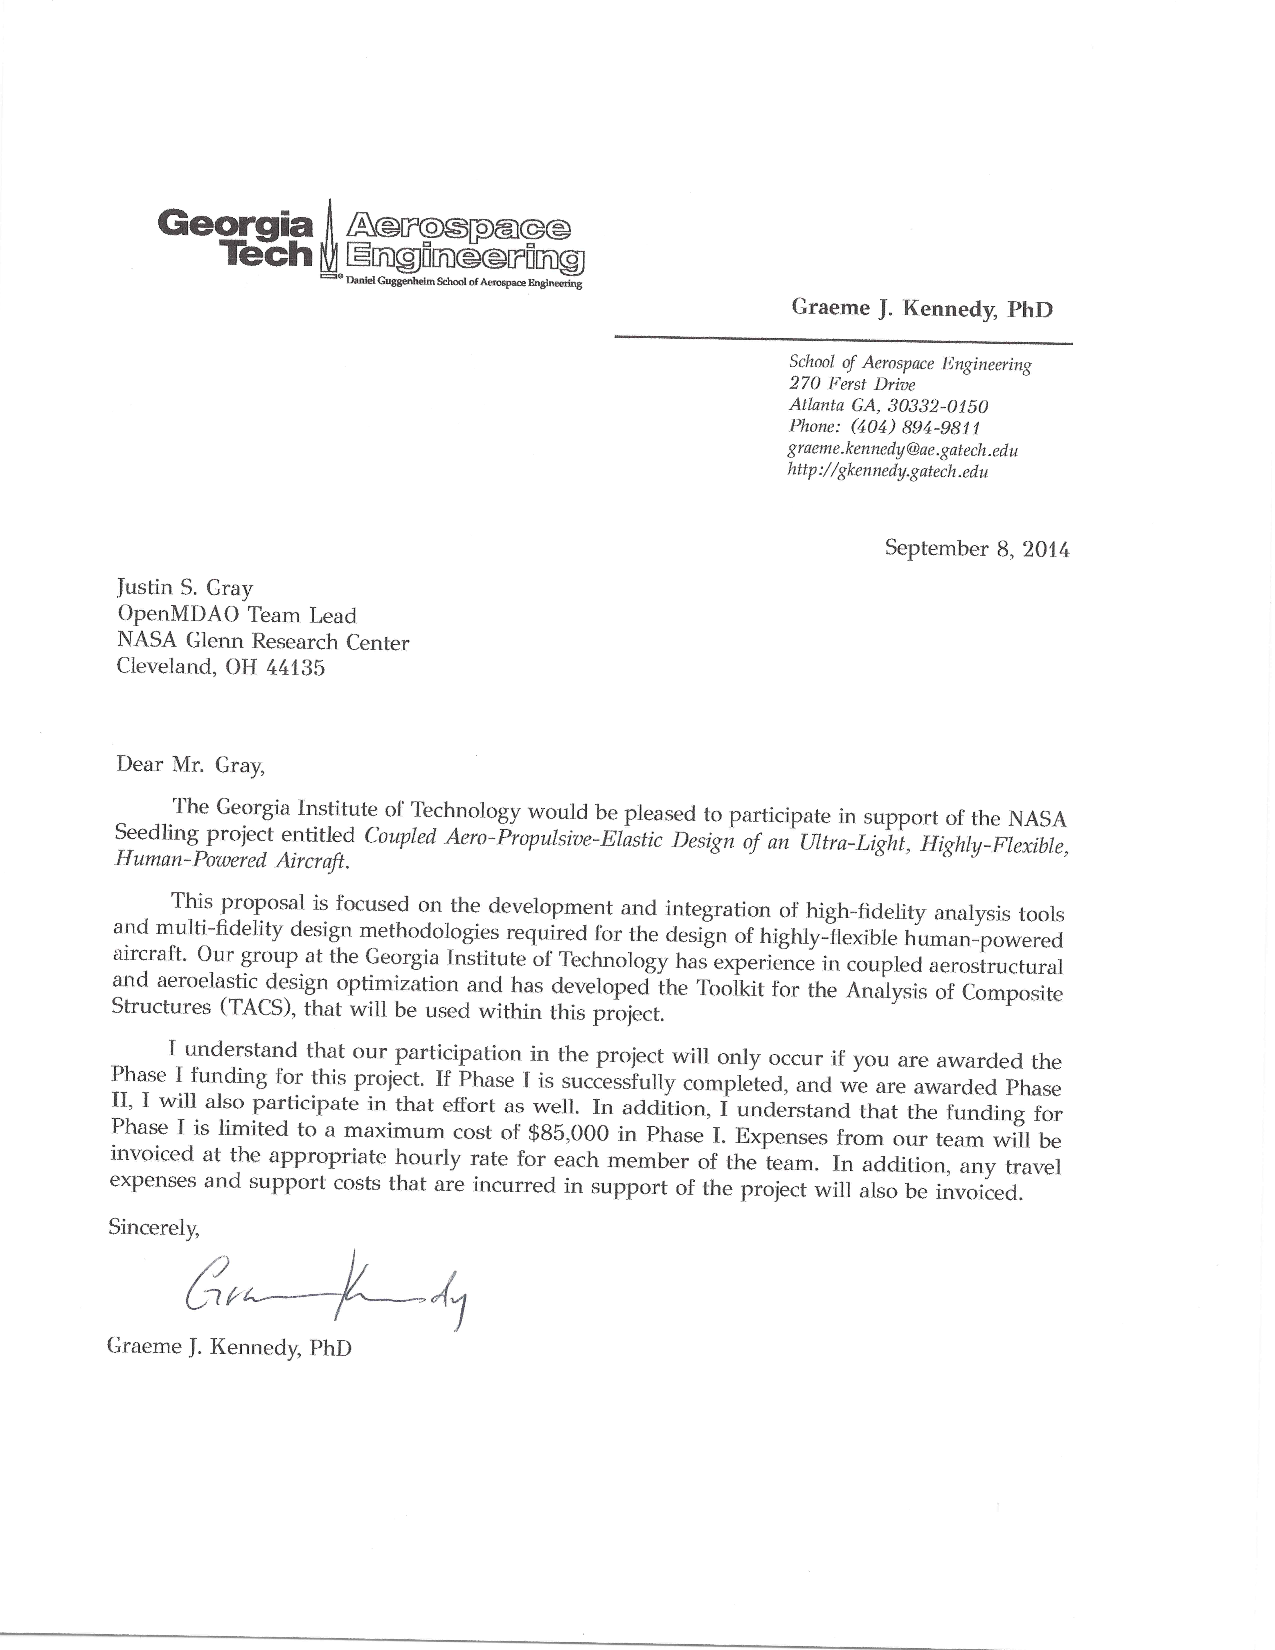
\includepdf[scale=1., pages={1}]{letters_of_commitment/gatech.pdf}
    \restoregeometry


  \section{Resumes \& Qualifications}

    \clearpage
    \newgeometry{left=0cm,bottom=0cm,top=0cm,right=0cm}
    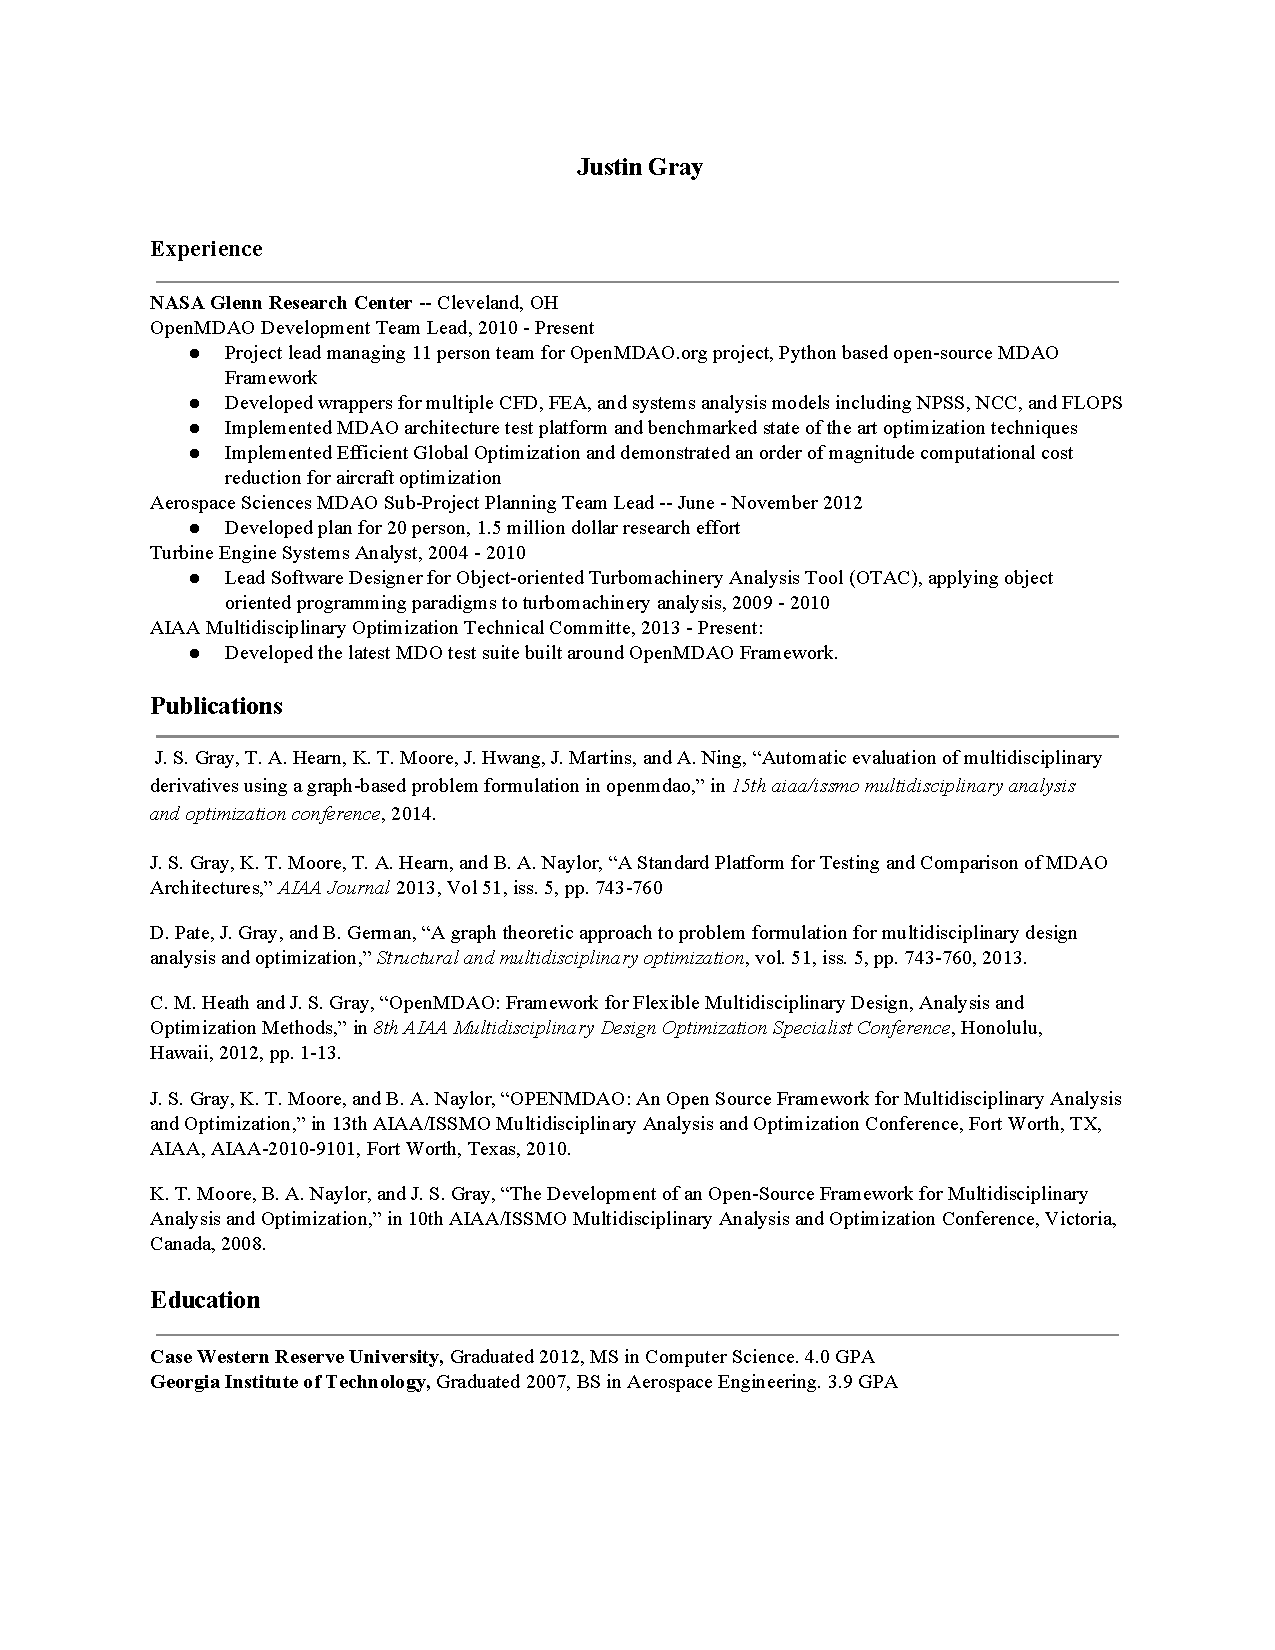
\includepdf[scale=1.2, pages={1}]{resumes/justin_resume.pdf}
    \restoregeometry
    \newpage
    \pagestyle{empty}

\noindent {\bf Juan J. Alonso} \\
Associate Professor \\
Department of Aeronautics \& Astronautics \\
496 Lomita Mall, Durand Building, Room 252 \\
Stanford, CA 94305 \\
Phone: (650) 723-9954, Fax: (650) 725-3377, jjalonso@stanford.edu \\

\noindent {\bf PROFESSIONAL CREDENTIALS } \\
Massachusetts Institute of Technology,  Aeronautics \& Astronautics,            B.S., 1991  \\
Princeton University,                   Mechanical \& Aerospace Engineering,    M.A., 1993  \\
Princeton University,                   Mechanical \& Aerospace Engineering,    Ph.D., 1997  \\

\noindent {\bf ACADEMIC / PROFESSIONAL APPOINTMENTS}  \\
2004-present, Stanford University, Associate Professor \\
2006-2008, NASA Headquarters, Director, NASA Fundamental Aeronautics Program  \\
1997-2004, Stanford University, Assistant Professor  \\
1996-98, McDonnell Douglas Corporation, Aerodynamic Designer  \\

\noindent {\bf AWARDS } \\
2013 Balhaus prize Ð Advisor for best doctoral thesis in Aeronautics \& Astronautics \\
2010 Altitude World Record, Class U, Unmanned Aerial Vehicles, Electric.  Advisor \\
2009 NASA Exceptional Public Service Medal\\
2006 F.W. Baldwin Award for best paper published in the Canadian Aero \& Space Journal\\
2004, 2006, 2008 AIAA Best Paper Award, Multi-Disciplinary Optimization Conferences\\
AIAA Stanford Chapter Professor of the Year (7-time recipient during the 1998-2013 period) \\
2003 Balhaus prize Ð Advisor for best doctoral thesis in Aeronautics \& Astronautics\\
1998-99 Stanford University Terman Fellow\\
1996 Ray Grimm Memorial Price in Computational Physics\\
1995-96 Princeton University Honorific Fellow\\
1992 Speed World Record, Human-Powered Vehicle Over Water.  Team member\\
1990 Admiral Luis de Florez Award in Mechanical Engineering Design\\

\noindent {\bf COMMITTEE/ADVISORY COUNCIL MEMBERSHIP } \\
2013-present, AIAA AVIATION Executive Steering Committee\\
2013-present, Associate Editor, Computers \& Fluids\\
2013-present, INRIA Evaluation Board Member\\
2012-present, AIAA Associate Fellow\\
2012-present, DLR Institut fŸr Lufttransportsysteme Advisory Board\\
2012-present, ICCT Technical Advisory Group member\\
2011-2012, FAA AdministratorÕs Management Advisory Council\\
2010-present, Secretary of TransportationÕs Future of Aviation Advisory Council\\
2009-present, CGNS (CFD General Notation System) Advisory Committee\\
2009-2010, ICAO/CAEP Independent Expert Group for Aircraft Fuel Burn Goals/Regulations\\
2007-2009, IMDEA (Mathematics), Scientific Advisory Committee Member\\
2007-present, Stanford PSAAP / PSAAP 2 Center Steering Committee\\
2006-present, FAA REDAC, Office of Energy and Environment  \\
2005-present, Center for Turbulence Research Steering Committee \\
2005-07, NASA Advisory Council (Aeronautics Committee)  \\
2006-08, VAATE Steering Committee\\
2006-08, Fixed-Wing Vehicle Council Member\\
2004-06, AIAA Multi-Disciplinary Optimization Technical Committee\\

\noindent {\bf RECENT SELECTED / RELEVANT PUBLICATIONS}

\begin{enumerate}

\item Hicken, J. E. and Alonso, J. J., ``PDE-Constrained Optimization with Error Estimation and Control,Ó Accepted for publication, Journal of Computational Physics, 2013.

\item Alonso, J. J., Bonnefoy, P. A., Bono, J., Fan, A., McConnachie, D., Tracey, B. D., Wolpert, D., Xie, D., ``Application of Game Theoretic Models to Evaluate Airline Equipage Dynamics of NextGen Technologies," 2013 Aviation Technology, Integration, and Operations conference, 10.2514/6.2013-4279

\item Shimoyama, K., Kawai, S., and Alonso, J. J., ``Dynamic Adaptive Sampling Based on Kriging Surrogate Models for Efficient Uncertainty Quantification," AIAA Paper 2013-1470, 54th AIAA/ASME/ASCE/AHS/ASC Structures, Structural Dynamics, and Materials Conference, 2013, 10.2514/6.2013-1470

\item Palacios, F., Alonso, J. J., Colonno, M., Hicken, J., Lukaczyk, T, ``Adjoint-based method for supersonic aircraft design using equivalent area distribution," AIAA Paper 2012-0269, 50th AIAA Aerospace Sciences Meeting including the New Horizons Forum and Aerospace Exposition, Nashville, TN, January 2012.

\item Palacios, F., Duraisamy, K., Alonso, J. J., Zuazua, E., ``Robust Grid Adaptation for Efficient Uncertainty Quantification," AIAA Journal Vol. 50, No. 7, July 2012.

\item Alonso, J. J. and Colonno, M., ``Multidisciplinary Optimization with Applications to Sonic Boom Minimization," Annual Reviews of Fluid Mechanics, vol. 44: 505-526, January 2012.

\item Tracey, B, Wolpert, D., Alonso, J. J., ``Using supervised learning to improve Monte Carlo integral estimation," AIAA Journal.

\item Choi, S., Potsdam, M., Lee, K., Iaccarino, G., and Alonso, J. J., ``Helicopter Rotor Design Using a Time-Spectral ROM and Adjoint-Based Method," AIAA Paper 2008-5810, 12th AIAA/ISSMO Multidisciplinary Analysis and Optimization Conference, Victoria, British Columbia, September, 2008.

\item Mader, C., Martins, J., Alonso, J. J., and van der Weide, E., ``ADjoint: An Approach for the Rapid Development of Discrete Adjoint Solvers," AIAA Journal, vol. 46, no. 4, pp. 863-873, April 2008.  Best paper award, AIAA Multidisciplinary Analysis and Optimization Conference, 2008.

\item Choi, S., Alonso, J. J., Kroo, I. M., and Wintzer, M., ``Multifidelity Design Optimization of Low-Boom Supersonic Jets," AIAA Journal, vol. 45, no. 1, pp. 106-118, January-February 2008.

\item Colonno, M., Reddy, S., and Alonso, J. J., ``Multi-Fidelity Trajectory Optimization with Response Surface Based Aerodynamic Performance Prediction," AIAA Paper 2008-0218, 46th Aerospace Sciences Meeting \& Exhibit, Reno, Nevada, January 2008.

\item J. R. R. A. Martins, J. J. Alonso, and J. J. Reuther. ``A Coupled-Adjoint Sensitivity Analysis Method for High-Fidelity Aero-Structural Design. Optimization and Engineering," 6(1):33Ð62, March 2005.  Best paper award, AIAA Multidisciplinary Analysis and Optimization Conference, 2004.

\item Reuther, J.J., Alonso, J.J., Jameson, A., Rimlinger, M.J., Saunders, D., ``Constrained Multipoint Aerodynamic Shape Optimization Using an Adjoint Formulation and Parallel Computers: Parts I and II," AIAA Journal of Aircraft, vol. 36, no. 1, pp. 51-74, January-February 1999.

\end{enumerate}

    \newpage
    \newgeometry{left=0cm,bottom=0cm,top=0cm,right=0cm}
    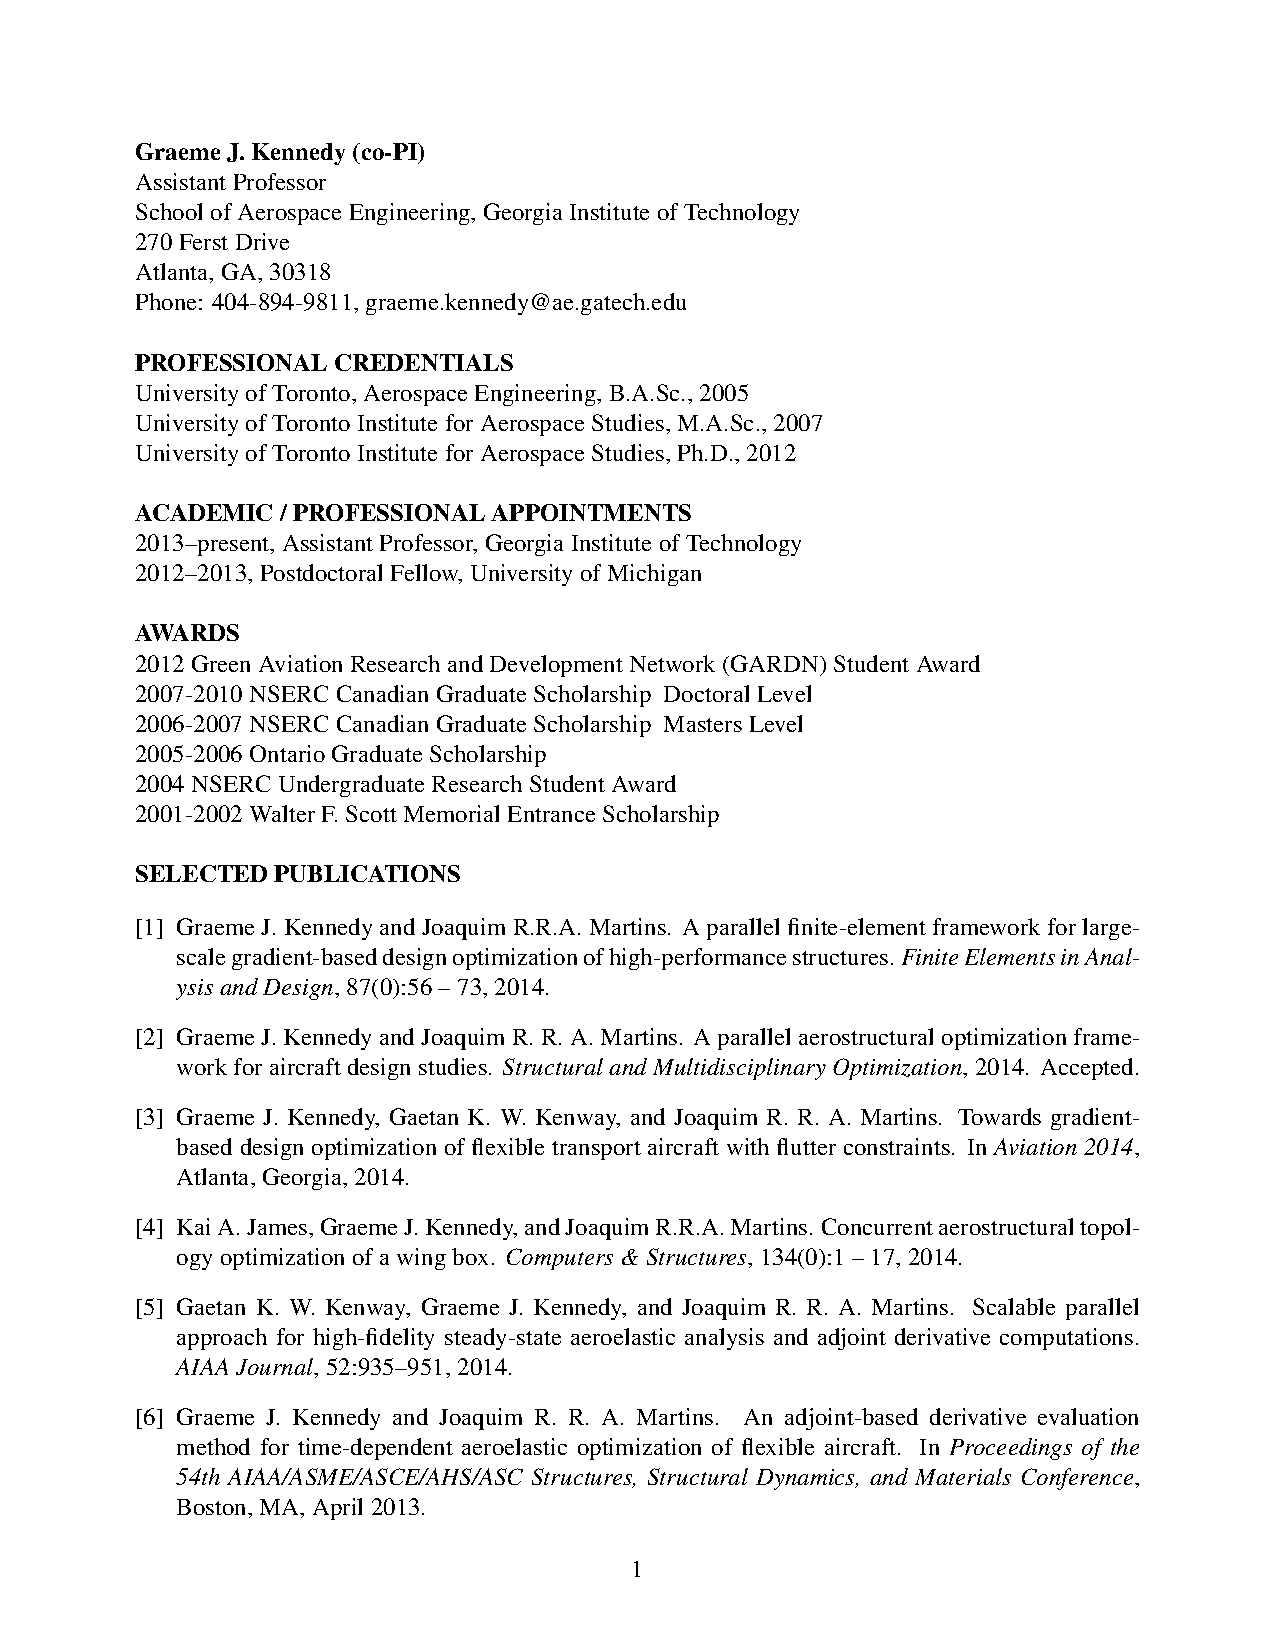
\includepdf[scale=1, pages={1,2}]{resumes/bio_kennedy.pdf}
    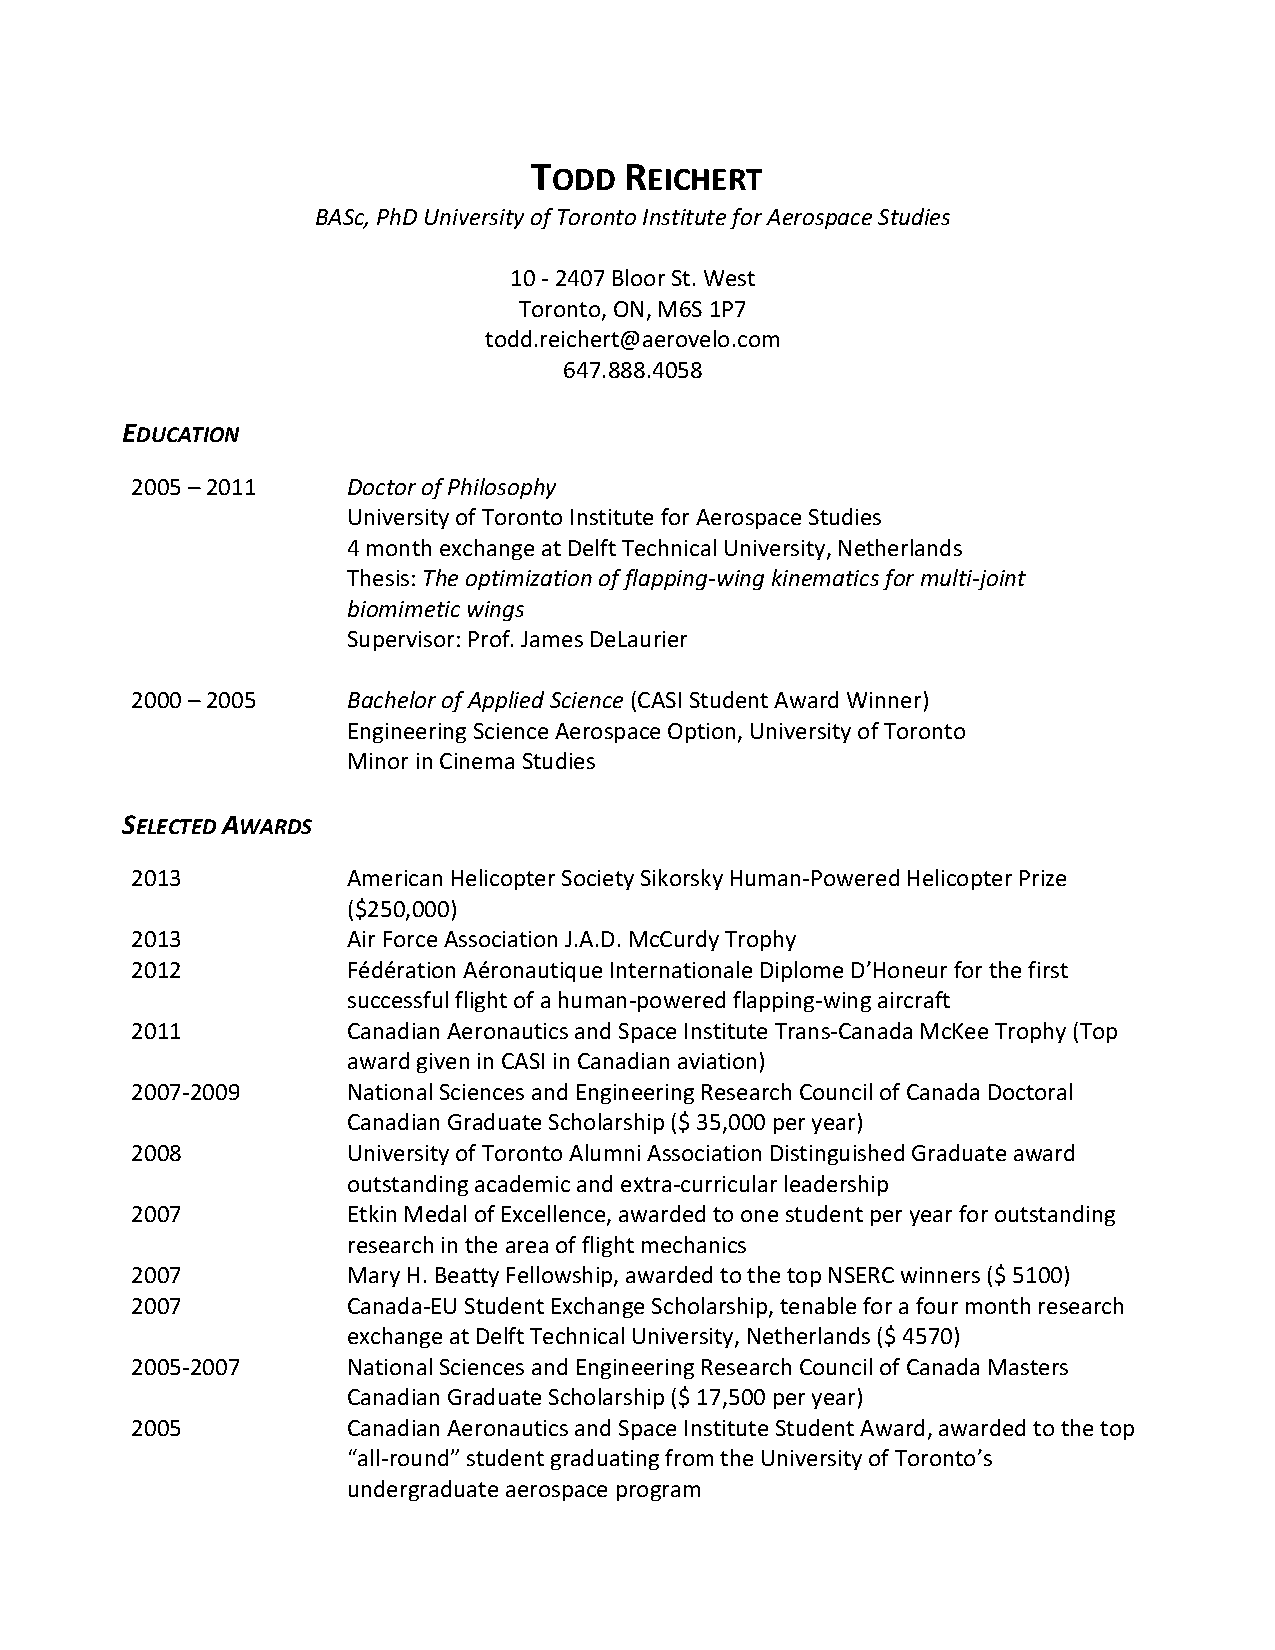
\includepdf[scale=1, pages={1,2,3}]{resumes/todd_reichert.pdf}

    \newgeometry{left=0.5cm,bottom=0cm,top=0cm,right=0.5cm}
    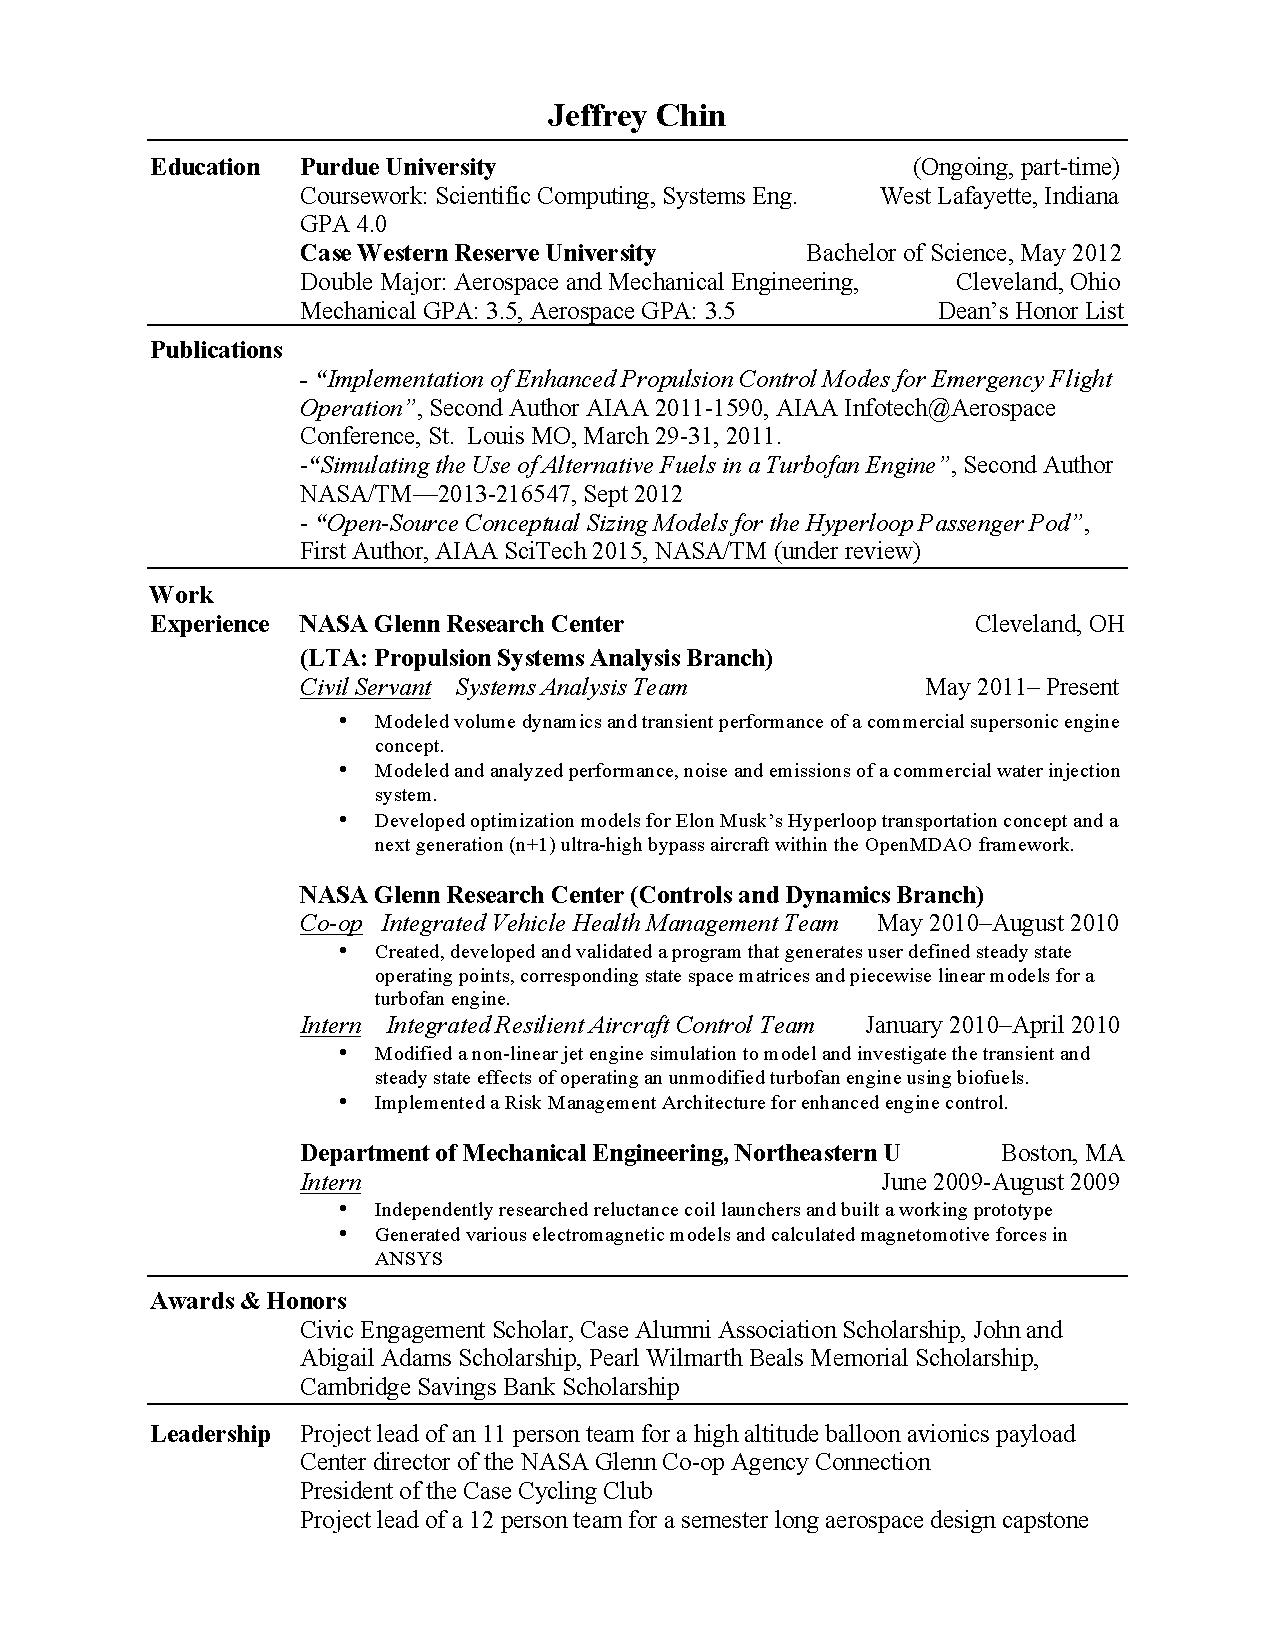
\includepdf[pages={1}]{resumes/Chin_SeedlingResume9_3_14.pdf}
    \newgeometry{left=0cm,bottom=0cm,top=0cm,right=0cm}
    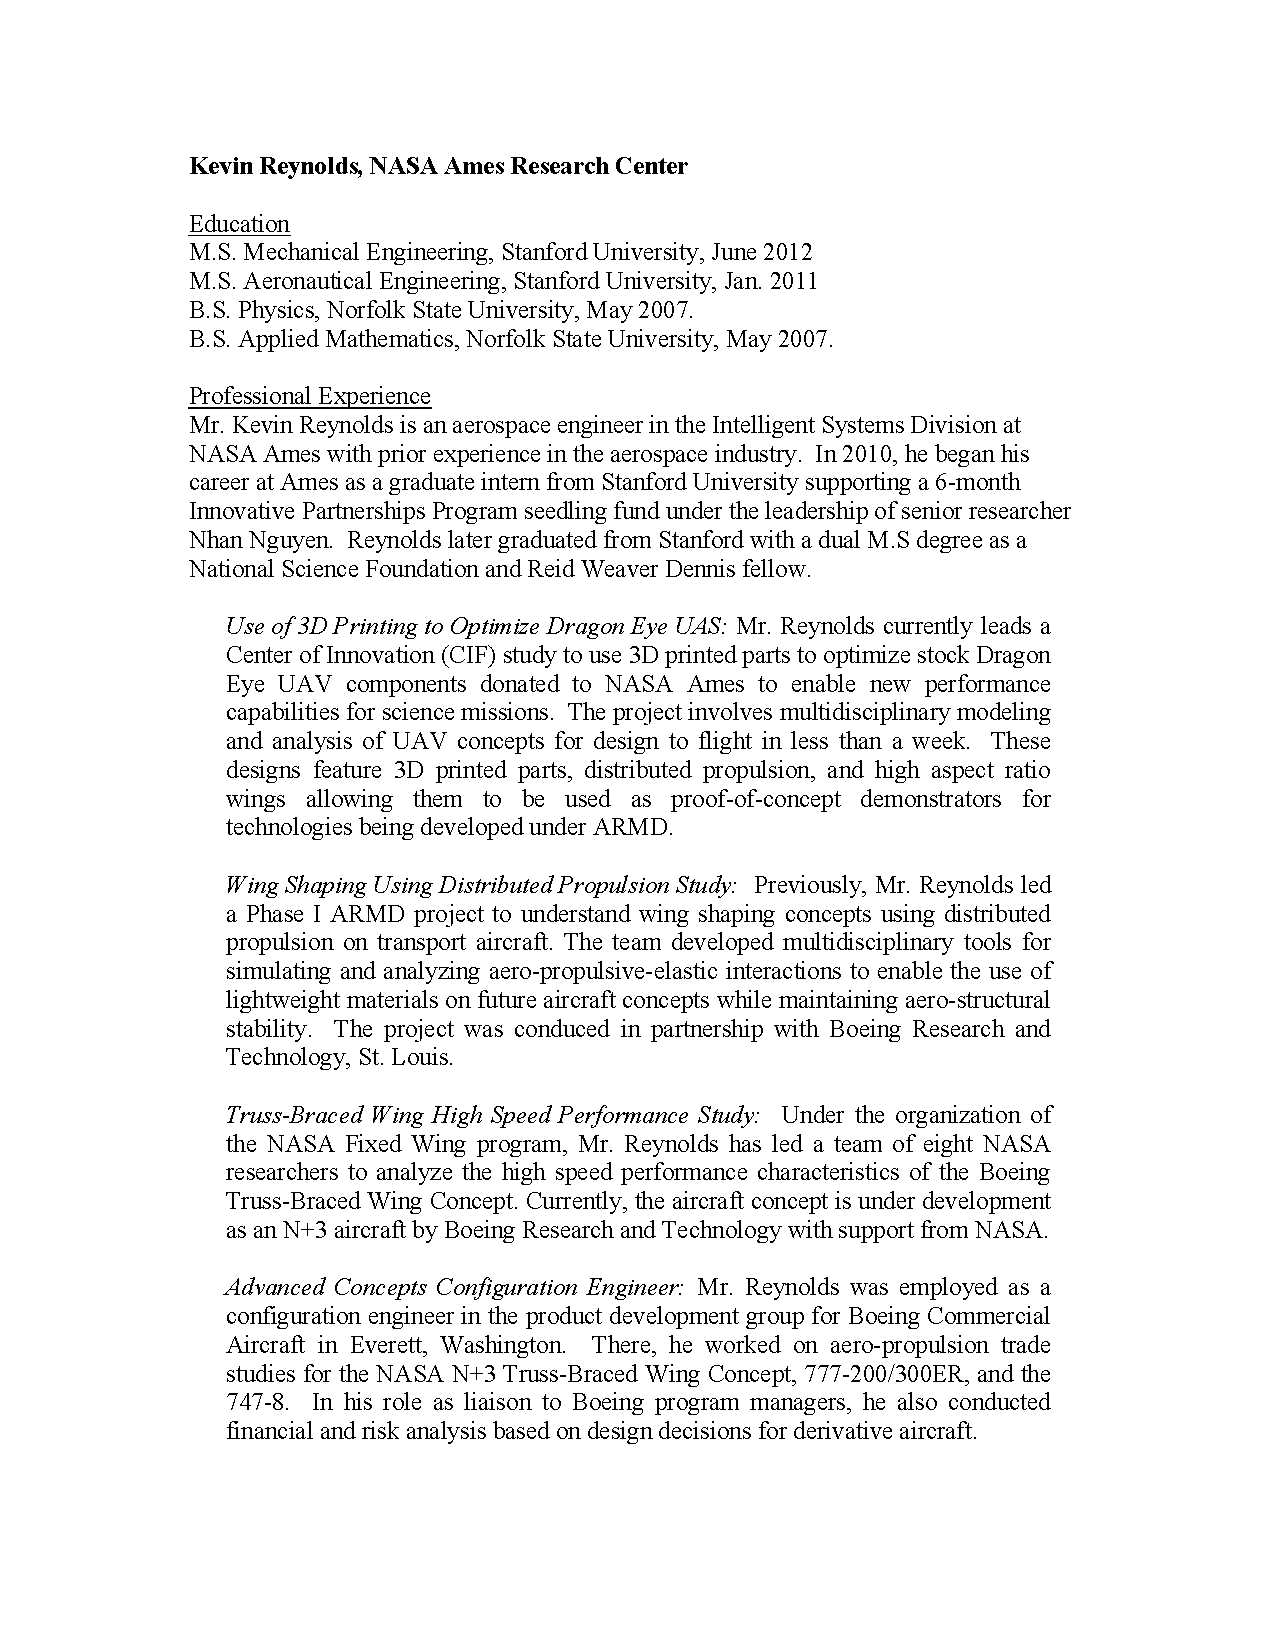
\includepdf[scale=1, pages={1}]{resumes/Kevin_reynolds_resume.pdf}
    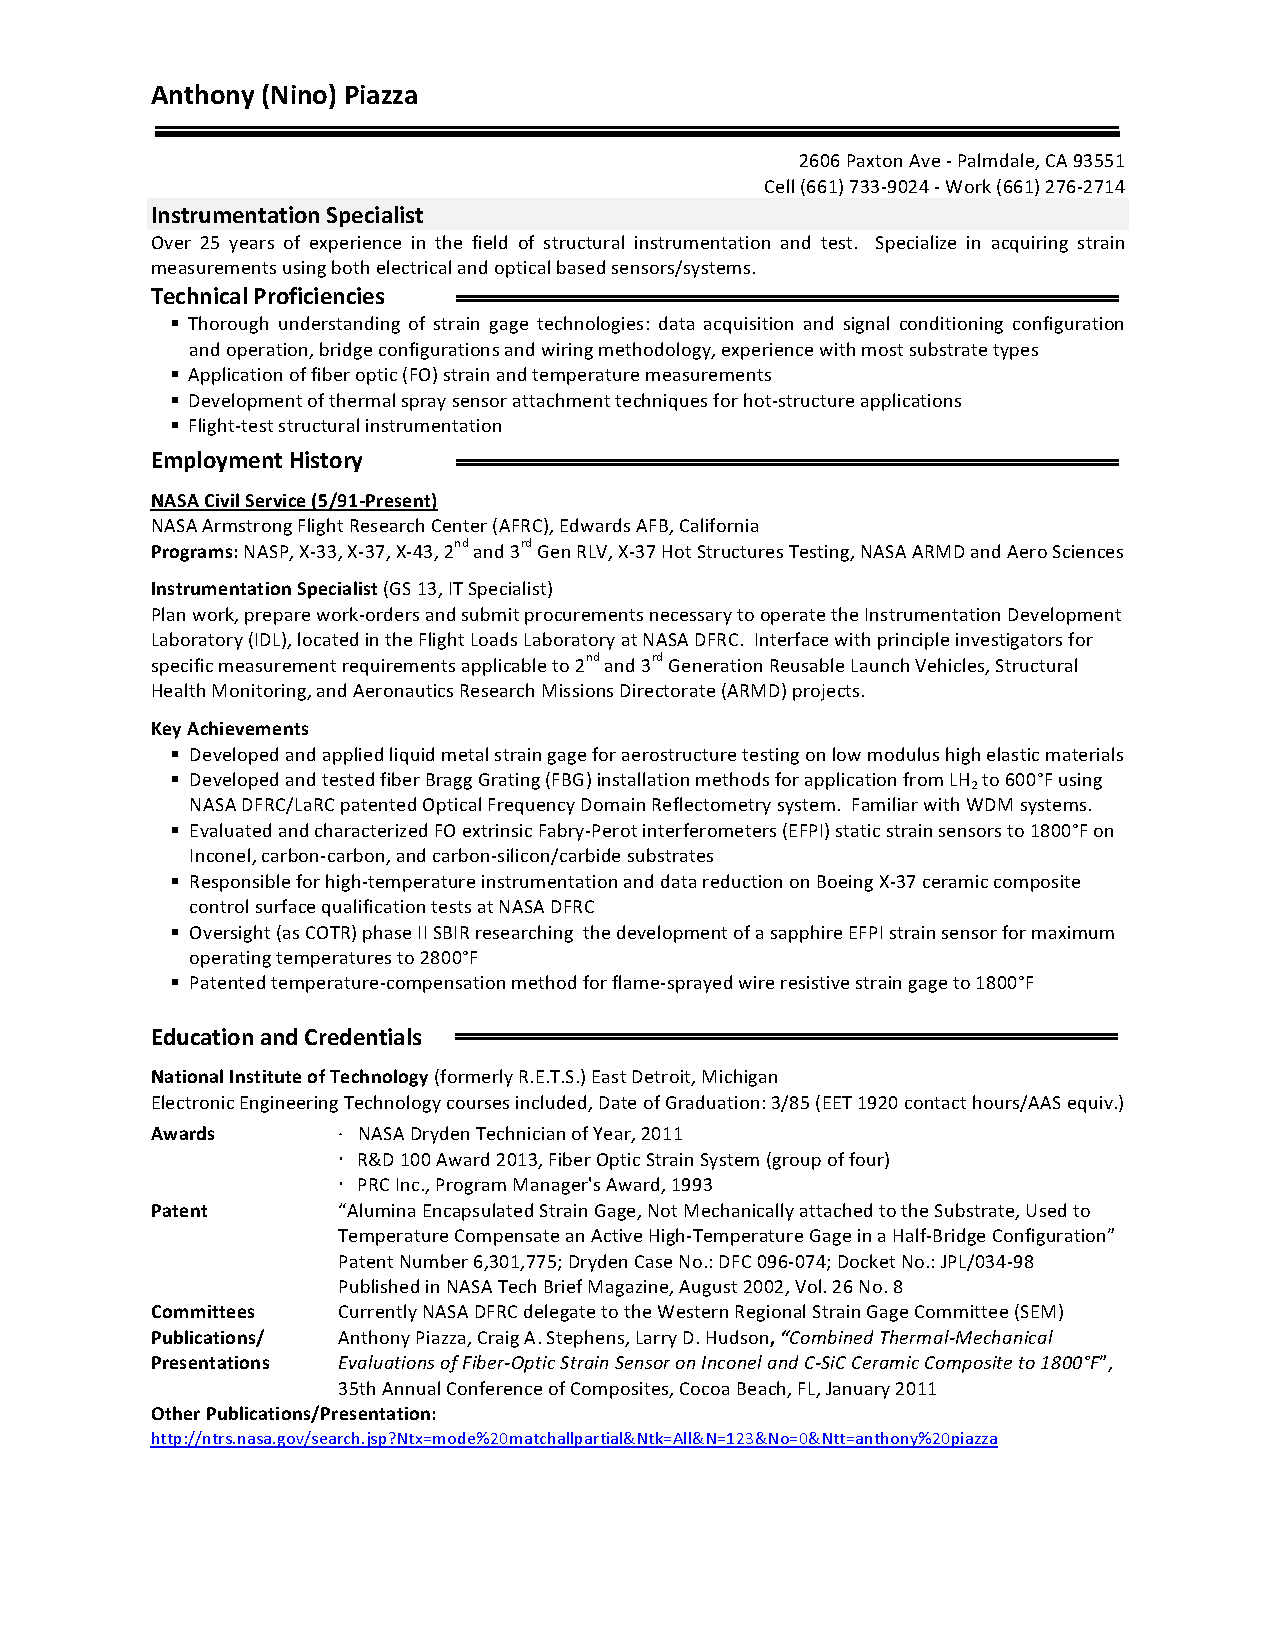
\includepdf[scale=1, pages={1}]{resumes/nino_piazza_resume.pdf}
   
    \restoregeometry



    

\end{document}
